% Chapter 6

\chapter{Further Experimentation and Comparative Analysis} % Main chapter title

\label{Chapter7} % For referencing the chapter elsewhere, use \ref{Chapter1} 

\lhead{Chapter 7. \emph{Further Experimentation and Comparative Analysis}} % This is for the header on each page - perhaps a shortened title

%----------------------------------------------------------------------------------------

\section{Introduction}

To make any data visualisation technique work, the data must be passed through four stages before being sorted and stored. These four stages are:
\begin{itemize}
\item 	Initial collection and mass storage of the data itself. This is the simplest phase and is easily performed independently of any kind of visualisation technique. It is pre-processing of the data. This stage is intended to transform the data and present it in a comprehensive form. By pre-processing the data applications, are then able to display the algorithms and work at a satisfactory and rapid rate, reducing the need to re-search the data file time and time again for more information.

\item	The data representation where the display hardware and software are used to produce a visual representation of the data. In an ideal world every implementation of a visualisation technique would be done using high performance display hardware and graphic libraries. Traditionally this would have increased the cost of visualisation, but the increase in performance efficiency and low cost of computing equipment, this is becoming more of a possibility.

\item	The next stage is the human interaction element. The algorithms used to visualise the data need to first address the limits of human perception. From there, the system needs to maintain these constraints whilst still presenting as much information as possible in an understandable format. These algorithms also need to understand that there are fine limits to the patience of human beings, and so the response time to queries is an important factor.

\item	The final stage is the storage of the data from the above three stages. 
\end{itemize}

In short, information visualisation is the process of users establishing a strong connection with a collection of data sets through a visual medium. Once the data has been processed by the appropriate system, it is displayed for human consumption in the form of charts and other visual media. Information visualisation has addressed many of the issues that have arisen in the field of data analysis recently, but it still have a long way to go. Current visualisation tools either focus entirely on one dimensional data and are not always well coordinated with multi-attribute data or business transactions to  work effectively. In any business analytical tool or information visualisation, the primary focus is always on the data. Simple visualisation models like the one shown in the abstract models Figure 1.2, are a more basic visualisation of data included in software packages, which serves the basic data visualisation needs. More complex visualisation models exist - and these are usually the result of extensive research (commonly at PhD level). These more complex models provide in-depth analysis, but are incredibly difficult to practice in an enterprise environment using real time data or with any business or non-business oriented applications. The proposed analysis model is based on an easy to use and integrate visualisation approach; visualisation aspects focusing on non-aggregated, multi-attribute, multiple dimension and multi-coordinate visualisation. This view is a novel contribution and a fresh approach to information visualisation, and one that will allow users to capitalise on the greatest strength of information visualisation tools. It will provide decision makers with the tools and data to identify the expected, discover the unexpected and understand the ebbs and flows. All of this can be achieved through the new proposed visualisation model. In this chapter, the model's four layers or stages are discussed with additional examples and discussion as its been explained in the last two chapters.

\section{Acquisition and Data Analysis}

The acquisition and data analysis stage of the information visualisation model holds a key role. It is the first step in the data analysis process, and prepares the raw data for processing by the representation in the visualisation model.


\subsection{Data Decisions at Enterprise Level}

In this case, the data set has been retrieved from a transactional data source, and contains delicate information about the company including sales, staff performance, sales figures, driver performance and work deliver-ability figures alongside operational information - all the information needed to create a unique and complete data set. The data set also represents a very specific date range, and due to the sheer amount of data consisting of several million data rows and columns, making it difficult to analyse manually. By exploring the data in new and innovative ways, it delivers new key insights to decision makers and end system users - thus helping users to find new trends, explore new patterns and gain a huge amount of knowledge from the data that would otherwise go unnoticed. Analysing the data in this way and gaining these insights, users are able to make smart business decisions and refine operations. The web intelligent agents have been specifically designed to operate within the enterprise environment where the data structure is known to the system and its supporting functions. Because the entity is already known, the system will automatically explore the data and find relationships between different attributes located in enterprise data sets. These data attribute relationships are based on various scenarios determined by studying business nature in detail. For example, a sales staff members performance should be related to both product and team sales attributes such as, which staff member sold what products. To analyse this, the system must determine what products are sell-able, and use this to determine who is the best at selling what products. Information about this data is already available, but it requires an analysis model to make sense of it and understand the relationships between the different attributes. This particular feature of the information computational model is closely related to multi-attribute information analysis.

\begin{figure}[H]
\centering
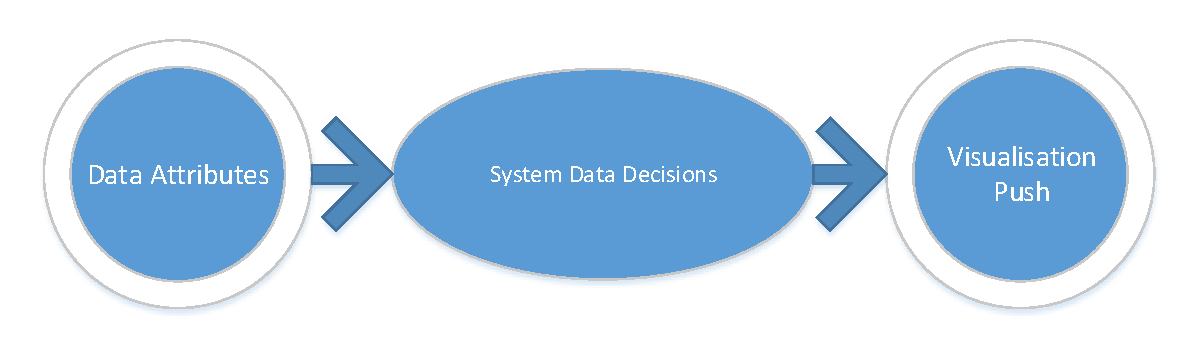
\includegraphics[scale=0.7]{chapter7/data_decisions}
\caption{System Data Decisions via Intelligent Agents }
\end{figure}


As shown in Figure 7.1, the data attributes are fed into the system, where these are analysed by the data analysis model in order to find relationships, which in turn lead to system data decisions. The system data decisions can be found through web intelligent agents, which in turn explore the relationships between different data attributes in detail. These relationships have been established and elaborated on, the data sets are then sent to the visualisation model, which visualises the data for the use of business managers and decision makers.

\subsection{Data Analysis at Non-Enterprise Level}

Data sets that are not in an enterprise environment from the start are processed by a different specialist tool, which was created for this type of research. The tool for this possesses the ability to read information from various sources and present through an import function. The import function then uploads the data sets into the indexation and processing model. In this model, data relationships are explored by the system and then categorised at the upper interface layer before visualisation takes place, giving the users and business managers the unique ability to select the various data attributes for visualisation.
 
\begin{figure}[H]
\centering
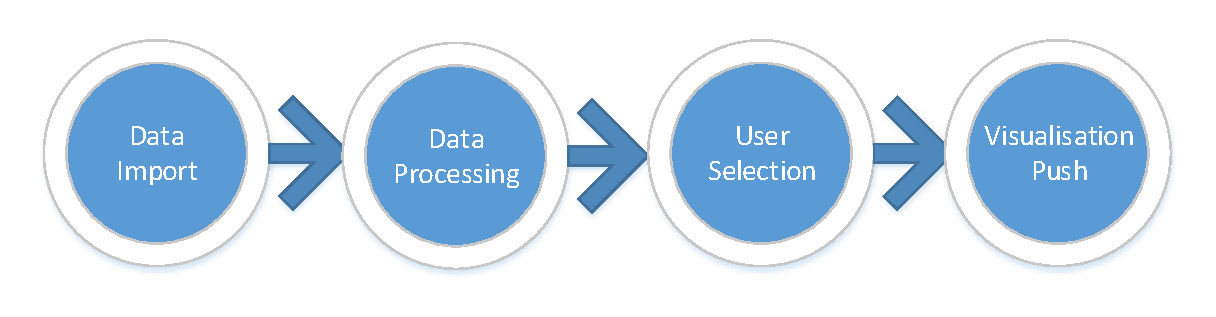
\includegraphics[scale=0.7]{chapter7/data_import}
\caption{Data Import Process in Data Analysis }
\end{figure}

As Figure 7.2 suggests, the data is imported into the data processing and indexing model through the simple and effective user interface. The data processing and indexing model than puts the data through a parsing process in order to find relations. Once it is housed, the user then has the ability to make data attribute selections. Once the relevant attributes are selected by the end user it is then pushed through to the visualisation model for graphic representation in the users chosen methods.

%Figure 7.3
\begin{figure}[H]
\centering
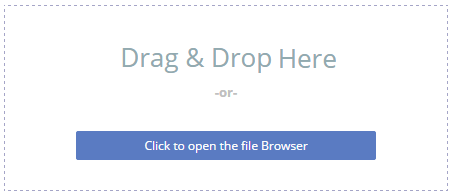
\includegraphics[scale=0.7]{chapter7/drag_and_drop_file}
\caption{Drag & Drop Files into Data Analysis Model }
\end{figure}

The important features of the system are the friendliness and ease of use, and the system utilises the file upload or drag and drop file approaches in order to create a smooth user experience as depicted in Figures 7.3 and 7.4. Once the files have been uploaded, the files are then forwarded to the data processing and indexation layer for further analysis.

%Figure 7.4
\begin{figure}[H]
\centering
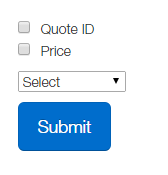
\includegraphics{chapter7/type_select}
\caption{Data Type Selection at User Interface }
\end{figure}

This simple user selection layer reads and analyses all the information from the data source, feeds it through a parsing process and then stores the information in a structural form within the system. The end users are then given the free choice to select the data and move it forward into the visualisation stage. Upon selection, the various data attributes are then moved to the visualisation model for the graphic representation stage.

\section{Data Representation}

Extensive research has been conducted in all four stages of the information visualisation process i-e (i) acquisition and data analysis, (ii) data representation, (iii) user interactivity and (iv) results repositories. However the proposed research and analysis techniques introduced at the represent++ layer is a predictive and analysis approach for data to explore data at different angles at same time, as this is where business owners find their business lacking in data analysis models. As shown in Figure 3.4, there are various different data representation techniques that are novel. The data representation layer is highlighted with selection of main visualisation types which are discussed in more detail below.

\subsection{Multi-coordinate Information Visualisation}

In terms of data analysis, multi-coordinate information visualisation is a specific exploratory visualisation technique which enables us to explore users data in ways which are extremely useful for the analysis purposes. In fact, the overall premise of this technique is that the end users are able to view and understand their data in a more succinct way, especially if it is presented in multiple views with additional interaction with data and the visualisation model. One of the main advantages of data visualisation is that users want to be able to look at their most complex and intricate data. Users want to be able to explore at their leisure and discover the facts and figures that aren't easy to find - as this is often what gives the edge in business. These more complex investigations of the data requires the user to consider multiple scenarios from different view points, and to compare visualisations that are generated from many different data sets. It is also able to aggregate and mine the data effectively - a task that is by no means a simple one, while also fusing data from multiple sources to generate new information and insights. On top of all of this - the user must also be able to roll back to the previous incarnation of the data in a few simple clicks.

Furthermore, many different business users might be looking at the same data sets in different ways, and might wish to compare and discuss the exploration paths and conclusions in different ways for different reasons. These analytic data investigations are often complex and  very long winded, and to carry out effectively the researchers must have at their disposal the right exploratory tools with comprehensive and intuitive functions to do the study justice. The information visualisation model also has the ability to analyse data of different types and sources from different angles within an enterprise environment through the intuitive use of mashup tools in an simple and easy to use approach. Because of this, business managers or end users can easily analyse the same data in various coordinated views. In other words, the same data set is visualised in different styles in order to understand and explore information, to gain  knowledge and new insights from incredibly complex data sets.

%Figure 7.5
\begin{figure}[H]
\centering
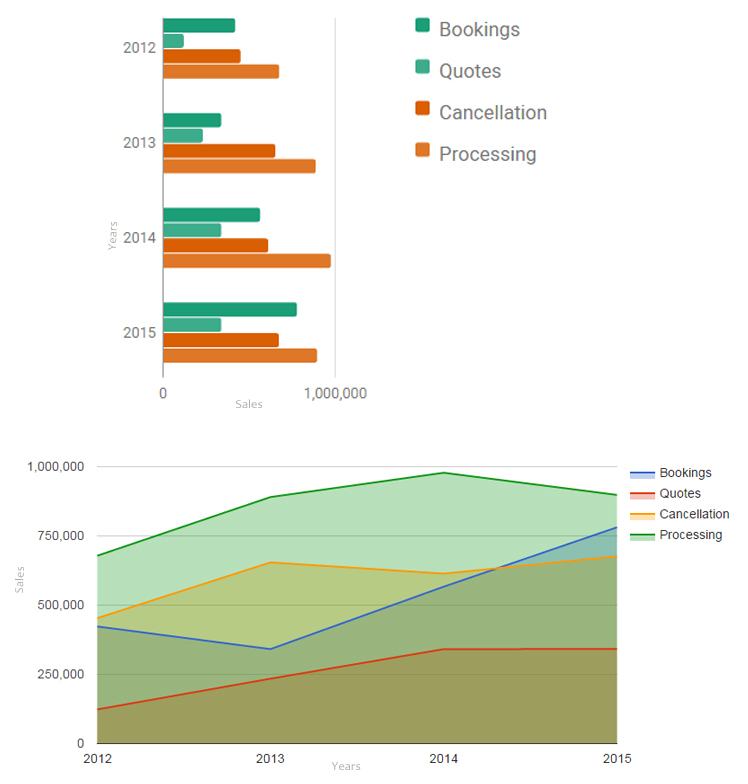
\includegraphics[scale=0.53]{chapter7/multi-coordinated1}
\caption{Multi-coordinate Information Visualisation}
\end{figure}

Figure 7.5 represents the same data visualised in two different styles, and allows the system to give more detail and depth of information to the end user. The bar graphs are indicating which staff member within the extracted data set leads the list. The area chart shows same data but in a different style. This approach gives plenty of options to users to analyse data from different angles. These various different data representations lead to an interesting variety of trends and patterns which cannot be understood in any other form of data representation.

%Figure 7.6
\begin{figure}[H]
\centering
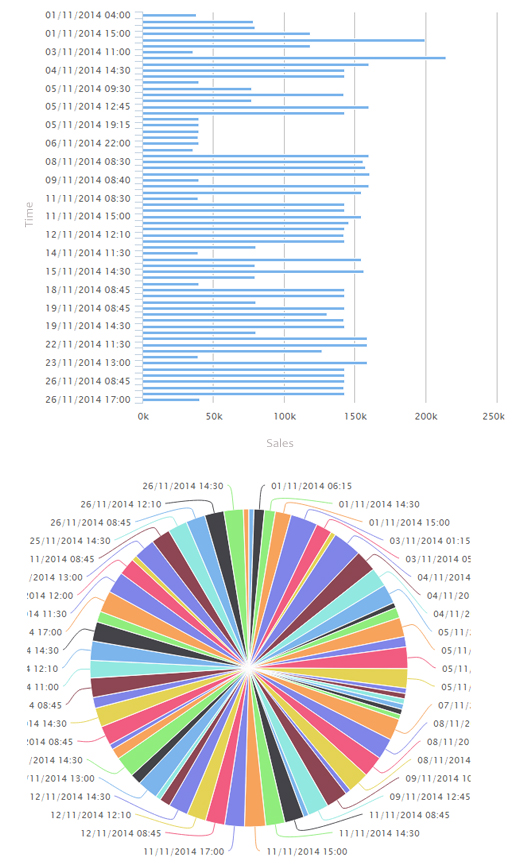
\includegraphics[scale=0.6]{chapter7/multi-coordinated2}
\caption{ Different Data View with Multi-coordinate Visualisation}
\end{figure}

The multi-coordinate information approach as demonstrated in Figure 7.6, is utilised by some applications, but oddly very rarely found in mashup systems, and even more rarely in the enterprise environment. It is incredibly effective in giving decision makers the ability to analyse data from various angles, and it is this that makes the proposed system unique and separates us from many other existing practice.

\subsection{Multiple Dimension Information Visualisation}

When a data set contains extremely large quantities of data, this can present a challenge for analysis. Attempting to analyse this type of data on its raw form to discover relationships and trends is a daunting if not completely difficult task. However, the proposed information visualisation model is focused exploring and finding aspect and forms where data could be represented to make more meaning out of the data. When the data being analysed is of a higher order (or a multiple dimension nature), limitations start to arise as the data becomes more and more complex. There are existing techniques for visualising this kind of high order data and allow it to be useful, but there is a mixed response as to whether the techniques are limited to the origin domain of the data being analysed \cite{keim2002information}. Users also run into trouble when analysing larger amounts of data, mainly that the visualisation process becomes messy and unclear the larger the data set becomes. As with any form of visual depiction, the message conveyed is generally open to interpretation.

%Figure 7.7
\begin{figure}[H]
\centering
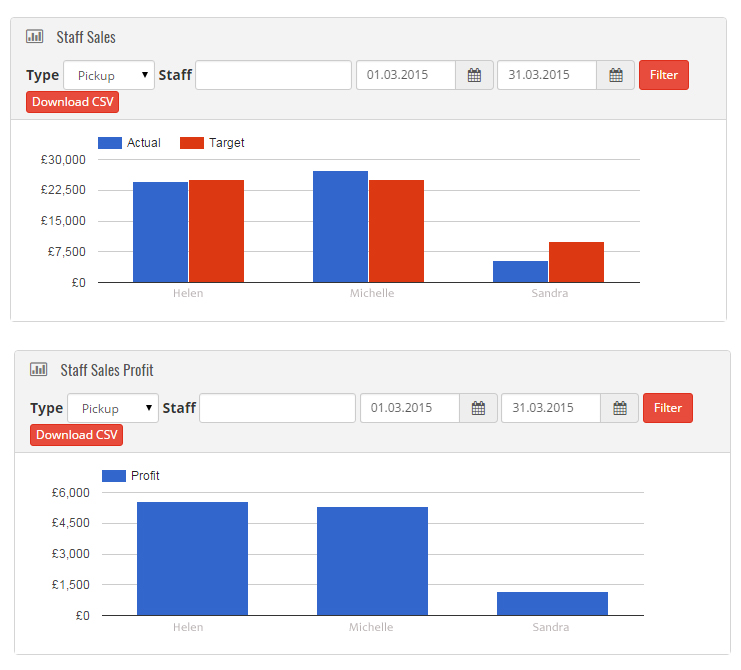
\includegraphics[scale=0.5]{chapter7/multiple_dimensional}
\caption{Multiple Dimension Information visualisation}
\end{figure}

Figure 7.7 depicts the data set discussed in visualised form, but the data has been explored further in order to find its dimensions. The bar chart shown at the top highlights team sales for a specific period, while the other chart shows profit generated by each staff member. The multi-dimension and multi-coordinate visualisation techniques help the decision makers to analyse real time data from different perspective. In this example, the decision makers can see, how much revenue was generated by a staff member while at same time, business profit against each staff member is shown. This is a quite unique approach to data visualisation, and the user will be able to get an idea of what products are sold, and which are undersold. This will help the business owner to focus on its most demanded resources while finding ways to better utilise resources that are not selling to their full potential.

\subsection{Multi-attribute Information Visualisation}

Many of the most interesting data sets within visual analytics come in the form of one or more multi-dimension relational tables. These data sets often include a mix of geo-spatial, temporal, numerical and categorical information \cite{grundy2009visualisation}. Nonetheless, multi-attribute graphs tend to be predominantly nominal in nature - mainly consisting of multiple dimensions of people, place, events, institutions, ideas and other kinds of names, entities and groups that represent the who and what of the social, political, legal and other human systems that are fairly complex.

The general structure of a typical attribute relationship graph consists of  well known visualisation components: 
\begin{itemize}
\item 	Dimensionally appropriate views for analysing the unique values of each attribute.
\item	Check boxes for toggling and filtering between any directed pair of views.
\item	A graphical view that shows values and value co-occurrences.
\item	Check boxes which toggle the filtering nodes for each different attribute, edges for each undirected attribute pair and hyper-edges for each directed attribute pair.
\end{itemize}

This intricate structure supports a complex process in which trained analysts can follow even the most complex lines of inquiry by using sequences of simple, freely interwoven interactions in order to perform specific visual data exploration and analytical tasks.

The attributed relational graphs have been used to define visual languages. The visualisation of attributes and relational data has also been noted as important yet largely overlooked from a systematic perspective, despite many examples of domain specific visual tools that include an interactive multiple graph representations.

%Figure 7.8
\begin{figure}[H]
\centering
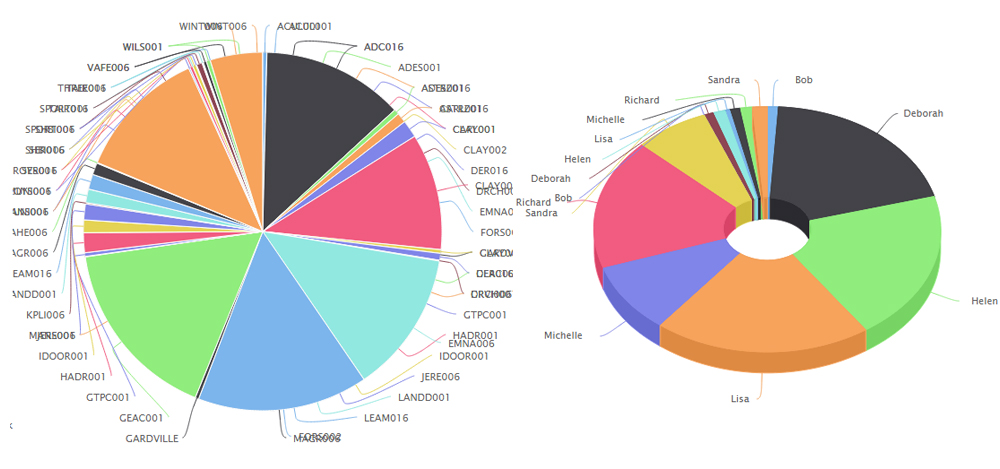
\includegraphics[scale=0.41]{chapter7/multi-attribute1}
\caption{ Example 1 Multi-attribute Information Visualisation}
\end{figure}

Figure 7.8 shows multi-attribute data visualised in a multi-coordinate view and showing different information. The left hand side pie chart shows customer accounts data. The pie chart on the right hand side showing staff member data. These two charts are related to each other through customer and staff data. The staff member figures (sales transactions) are shown on the right had side while the same sales transactions are further visualised and showing customers whom these transactions are related.  Multi-attributes information visualisation is a useful practice for cross data examination. Another example of the multi-attribute data is depicted in Figure 7.9.

%Figure 7.9
\begin{figure}[H]
\centering
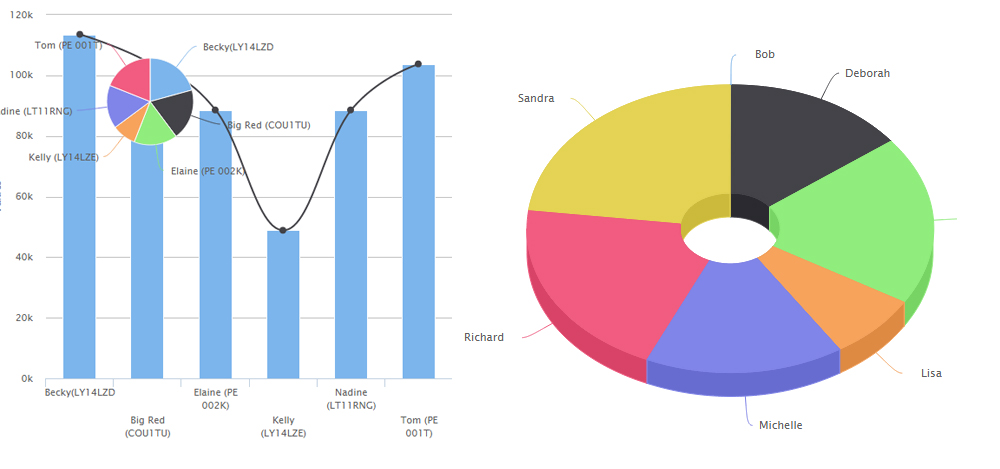
\includegraphics[scale=0.41]{chapter7/multi-attribute2}
\caption{ Example 2 Multi-attribute Information Visualisation}
\end{figure}

\subsection{Transactional Tagging Visualisation}

Transactional tagging visualisation is the name of the proposed approach, and will visualise tagged information within the data set. The end user will have the option to visualise both system tagged data and manually tagged data in the same space. In the charts above, the collected data is visualised and examined from the business transactional data set, tagged automatically by the system while exploring links and relationship, however this could also be tagged manually by a user and entered into the system. In Figure 6.6, an attempt to visualise the same information in a bubble chart with tags is illustrated. The graphs demonstrated in Figures 7.10 and 7.11 are generated with transactional tagging approach with extracted information from the whole data set for a limited data period. The tagged data visualised through tree map graphs shows interesting trends. The business managers can see what areas of the their business are successful.

%Figure 7.10
\begin{figure}[H]
\centering
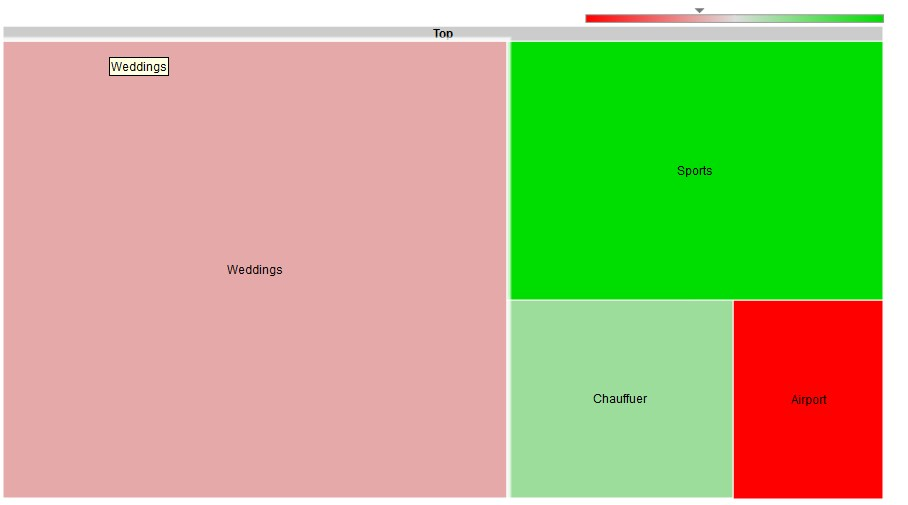
\includegraphics[scale=0.6]{chapter7/transaction-tagging3}
\caption{ Tagged-Data Treemap Top View}
\end{figure}

The graph has the ability to see sub-tagged information by clicking on the related part. Figure 7.11 suggests the areas where weddings orders are delivered.

%Figure 7.11
\begin{figure}[H]
\centering
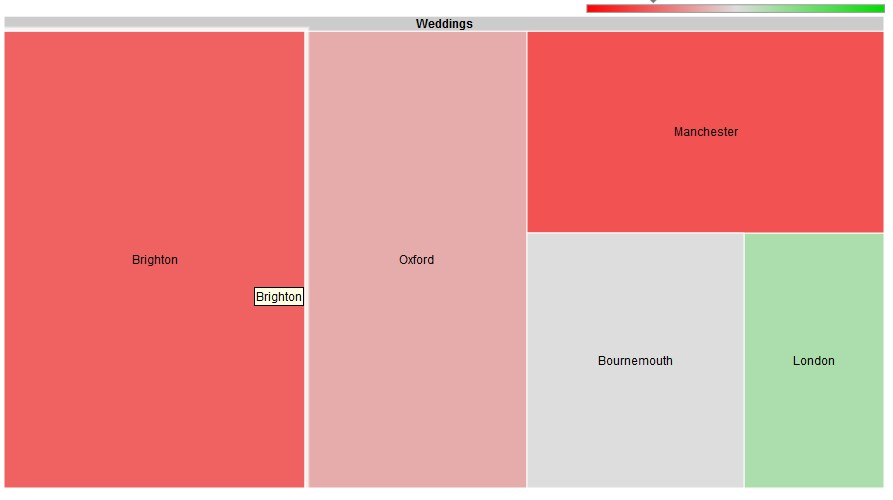
\includegraphics[scale=0.6]{chapter7/transaction-tagging4}
\caption{ Tagged-Data in Treemap Graphs}
\end{figure}

The transactional tagging is very new approach and gives additional information with quite different approach and understanding. This would play a vital role in shaping any business sales or operational modules. The transactional tagging was also explained in the previous chapter in experiment two. 

\subsection{Linked Data Information Visualisation}

The linked data approach was introduced by the creator of web Sir Tim Berners-Lee \cite{bizer2009linked}. Linked Data is more focused on the social and the overall data available over the Internet. Linked data focuses on elements of data which are related but not previously linked with its origin.

For instance, if a person has account with Facebook and the same person is also using Twitter. Then the information should refer to the same person. The linked data technique will find relation between two virtual accounts which lead to the same person in the physical world. Figure 7.12 illustrates LOD cloud diagram. This image depicts data sets that have been published in Linked Data format, by contributors to the Linking Open Data community project and other individuals and organisations. It is based on metadata collected and curated by contributors to the Data Hub as well as on metadata extracted from a crawl of the Linked Data web conducted in April 2014 \cite{linkeddata1}.

%Figure 7.12
\begin{figure}[H]
\centering
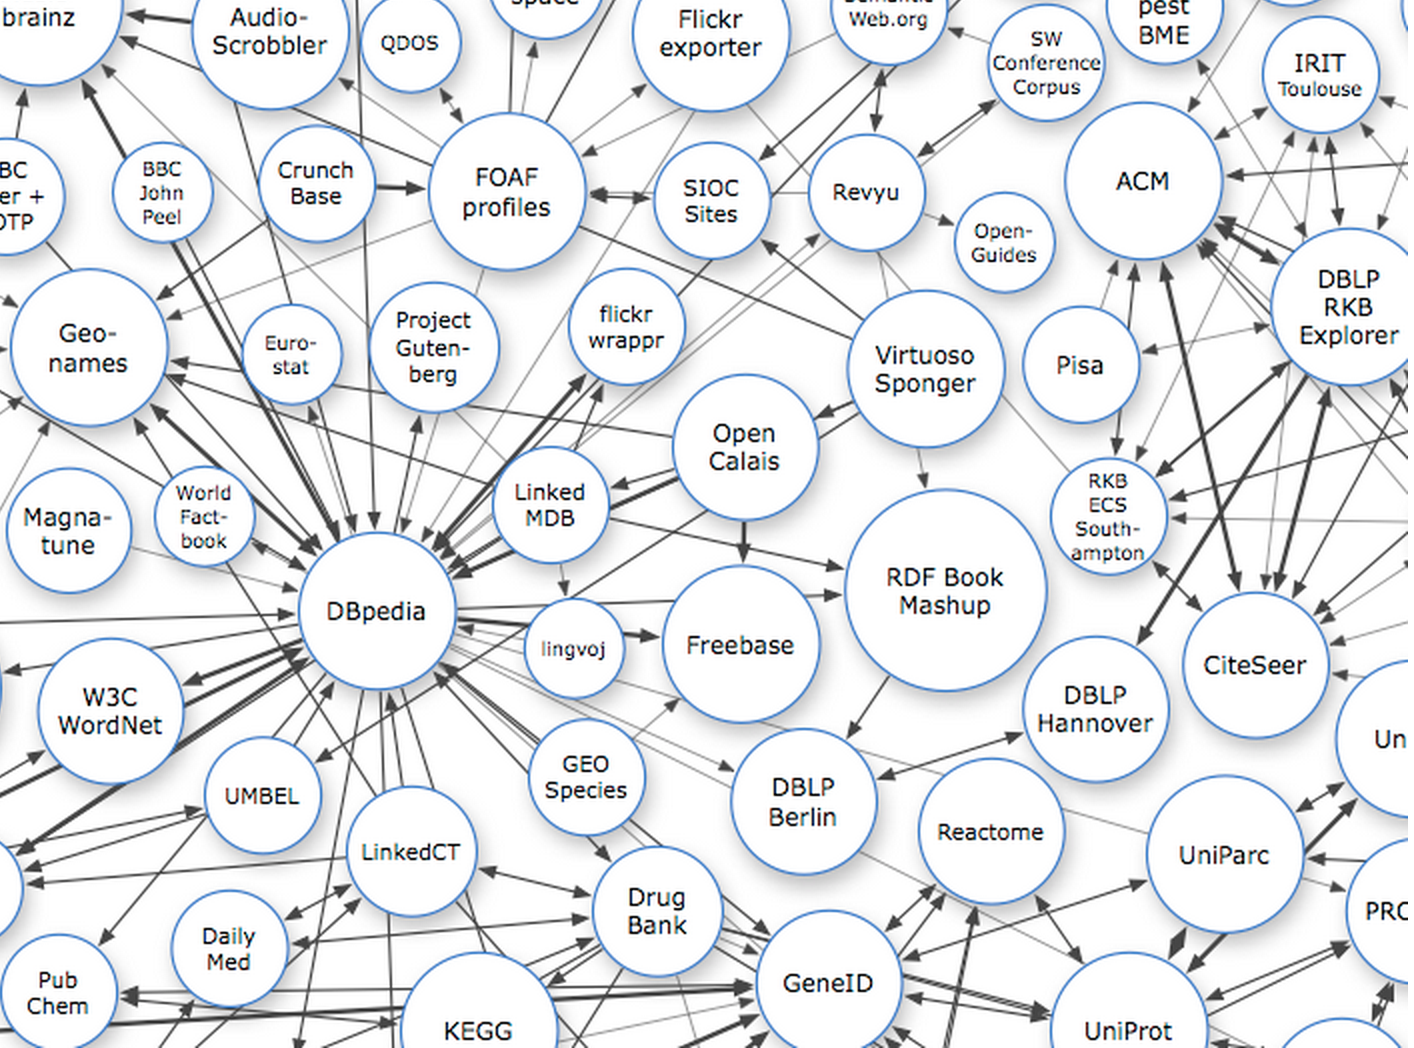
\includegraphics[scale=0.54]{chapter7/linked_data_new1}
\caption{Linked Dataset Visualised \cite{linkeddata1}}
\end{figure}

This concept has received appreciation from all walks of life. However, the same principle to find relationships between data could be applied in information visualisation to any commercial and non-commercial data set. Exploring relations are tedious work and will require a robust system to analyse and index data and review from different degrees for establishing the relationships. The initial proposal is to provide a procedure or system where data relations are explored by the system and presented to the end user through information visualisation.

The data set used in the experiment two in the previous chapter, has been used for linked data visualisation. The linked data visualisation works with multi-coordinate visualisation. The system find relations between data elements and then visualised in a multi-attribute and multi-coordinate views. Figure 6.6 shows, transactional tagging visualisation (with industry type highlighted) along with sales bar chart in a simple form. The sales chart shows button detail - which means the bar charts will be further divided into several sub elements as shown in Figure 7.13. The sub elements of the bar charts are data segmentation of data based on data element relation.

%Figure 7.13
\begin{figure}[H]
\centering
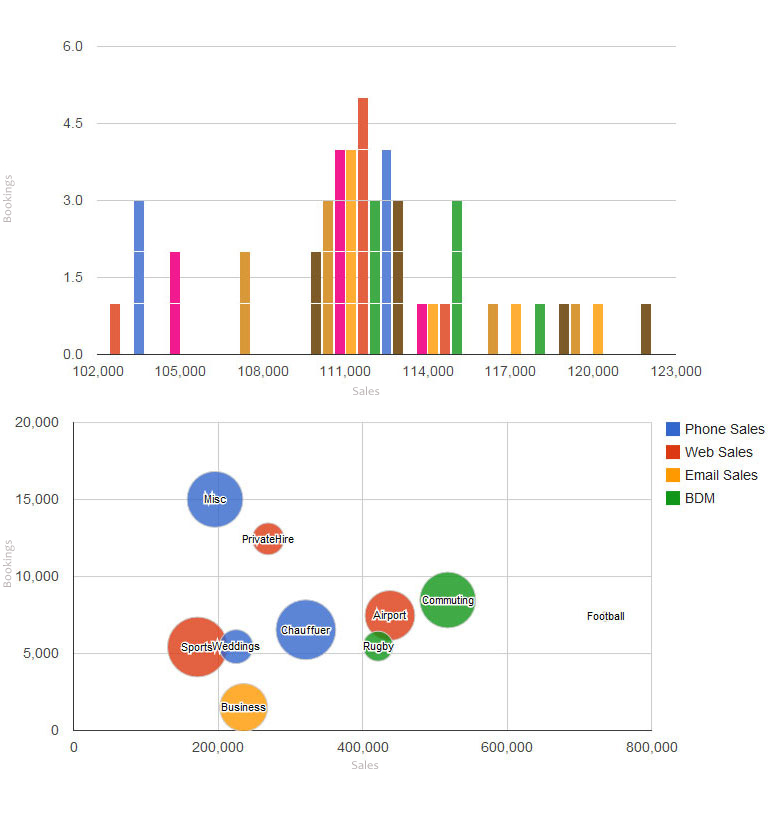
\includegraphics[scale=0.56]{chapter7/linkdeddata5}
\caption{Multi-coordinate with Detailed Bar Charts}
\end{figure}

As the detail sub bar charts are shown in Figure 7.14, if the user hover on any segment in the bar chart, the appropriate and related elements will be highlighted in the tagged data container. Thus giving additional information to user to analyse data. In this case, sales staff Lisa has sold £33K worth business bookings. The additional information is then shown through a pie chart in the interactive tool tip which was triggered by the relationship aspect between the two data segments.

%Figure 7.14
\begin{figure}[H]
\centering
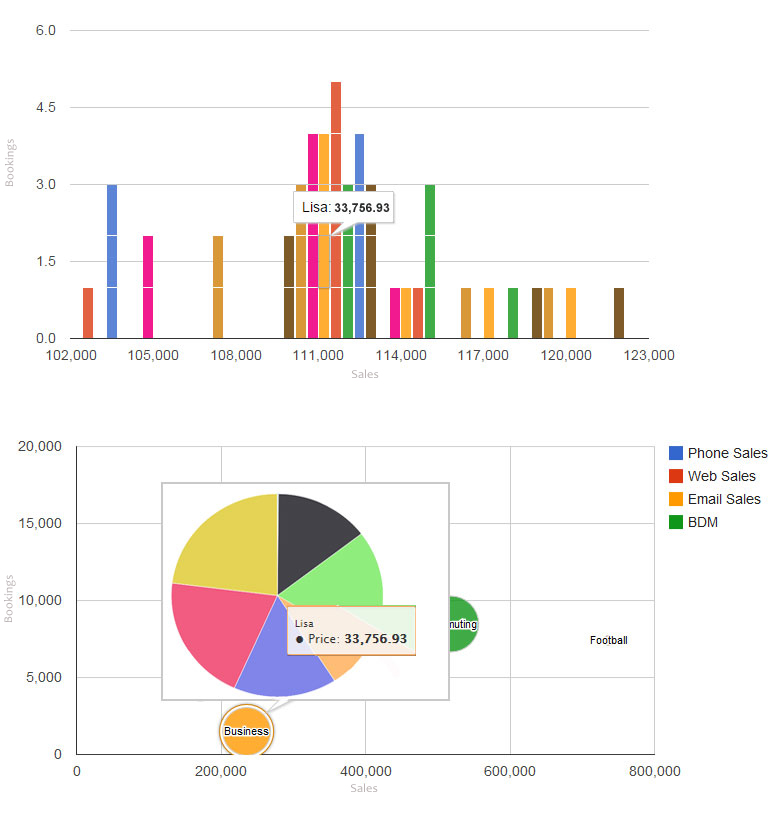
\includegraphics[scale=0.56]{chapter7/linkdeddata6}
\caption{Linked Data Visualisation}
\end{figure}

The above examples shows the importance of linked data visualisation, this new technique needs to be analysed further with more and variant data experiments. The next section explain user interaction with visualised data and with the system by giving instructions to the analysis model.

\section{Interactivity}

A mashup (in web development fields) is a web page or application that uses content from more than one source in order to create a single new service displayed in a single graphical interface. For example, users could combine the addresses and photographs in library branches with a Google map to create a unique map mashup. The term was chosen because it implies easy, fast integration, frequently using open application programming interfaces and data sources to produce enriched results that were not necessarily the original reason for producing the source data, but instead a complimentary option. The information visualisation model designed in this thesis has utilised various different mashup technologies in producing the output of data through various analysis models. Once the data has been processed by the system, it is made available to business managers and decision makers. These users have the ability to select various attributes of data from the system and cross examine it by using information visualisation techniques. For example - an individual user in a vehicle hire company could use the system and the visualised data to see what vehicle has been hired out, and to what location. This is the sort of attribute that the user could request of the system, before represented visually so we can see the graphical relationship between the two attributes pulled from the data set.

%Figure 7.15
\begin{figure}[H]
\centering
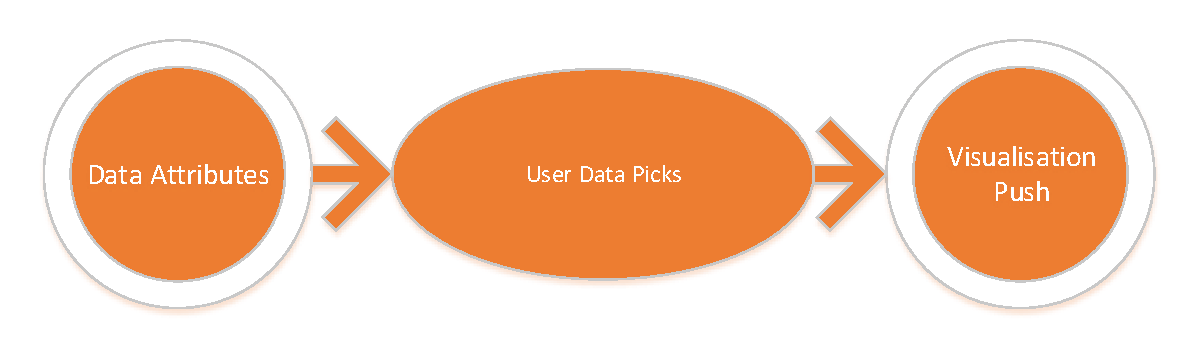
\includegraphics[scale=0.74]{chapter7/user_data_decisions}
\caption{Data Decisions by Users via Interface }
\end{figure}

Figure 7.15 shows that the required data attributes of the system are selected by the user and passed to the user data through data selection stage, where a series of web intelligent agents process data and prepare it for the represent++ layer. Web intelligent agents in this scenario are computer programs capable of processing different data attributes from the system and unearthing relationships, before passing the data on to the visualisation stage for transformation into graphically represented data. 

Approaches such as this are otherwise known as on-demand data visualisation practice. This process covers the steps of initial user request, the system selecting the data from the source and finally pushing the data to the visualisation stage, allowing it to be presented in visual form for further analysis.

\section{History}

The history layer both at the enterprise and non-enterprise level gives the ability to users to export information for external references or usages. This feature is very handy in giving the users the ability to extract useful visualised or non-visualised information in various formats such as JPEG, PNG, GIF and PDFS for external presentations and documentations. The next section shows comparison with existing tools and technologies in the same area. The first comparison is with the Fry \cite{fry} zipcode project and various other visualisation tools.

\section{System Comparison}

In this section, the three different experiments undertaken in this research will be compared with existing tools and technologies. In the first part, the UK postcode data set results will be compared with Fry \cite{fry} Zipcode project. The next part is comparison of business transactional data with various tools.

\subsection{UK Postcodes Vs Fry Zipcodes}

The information visualisation model takes the idea of postcode data and transforms it into an interactive map with multiple functionality layers for optimum data exploration. 

In the US, a postcode is known as a zipcode. The acronym ZIP stands for Zoning Improvement Plan, and refers to a 1963 initiative to simplify the delivery of mail within the United States \cite{mccurley2001geospatial}. Because the authorities were faced with an ever increasing amount of mail to be processed and delivered quickly, the introduction of the ZIP system was intended to simplify the process by more accurately specifying the geographic area. More information about the origin of the zipcode, user can read more on the US Postal Service's website \cite{uszipcode}. The zipcode database is available for general use, mainly through the US Census Bureau, who uses it as their primary method for the geographic coding of information. The listing is freely available to the general public.

%Figure 7.16
\begin{figure}[H]
\centering
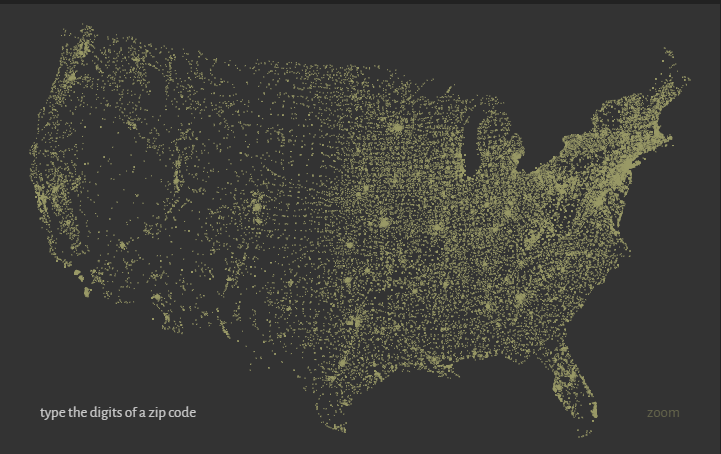
\includegraphics[scale=0.75]{chapter7/fry_zipcode}
\caption{Overview of Fry's Zipcode Map}
\end{figure}

When looking at the general representation of data, the main consideration is the basic form that the data set could take. Some data sets take the form of lists, while others are structured like trees. In this situation, each zipcode has a latitude and longitude to allow to be mapped as  a two-dimensional plot as depicted in Figure 7.16, with minimum and maximum values for the latitude and longitude used as the start and end points of the scale within each dimension. The zipcode data has been beautifully portrayed on a map of the US in Figures 7.16 and 7.17. The map is a static image representation and the data is overlaid to be presented on it in an interactive manner. For standard users who have a limited knowledge of the US and it's geography, it can be extremely difficult to know which zipcode represents what area, and what area belongs to which city. Moreover, there is much less interactivity for users in this form apart from typing in the postcode to show a highlighted area, as seen in Figure 7.17.

%Figure 7.17
\begin{figure}[H]
\centering
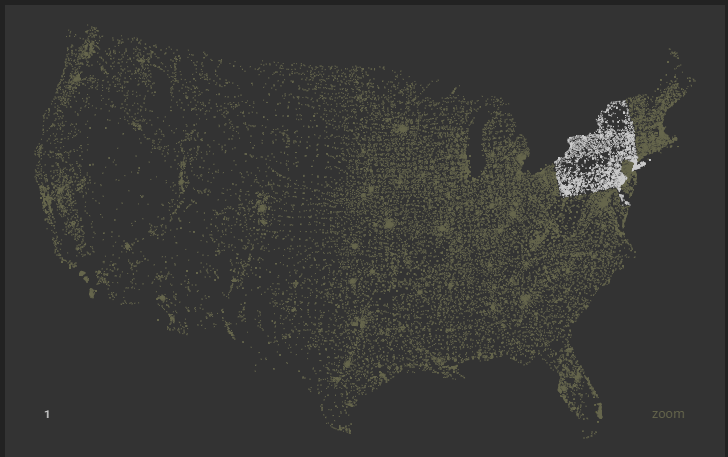
\includegraphics[scale=0.75]{chapter7/fry_zipcode2}
\caption{Highlighted Veiw of Fry's \cite{fry} Zipcode Map }
\end{figure}

In Figure 7.17 the focused area of searching is highlighted beautifully for users, where the zipcodes that start with the number 1 are located within the geographical area.

%Figure 7.18
\begin{figure}[H]
\centering
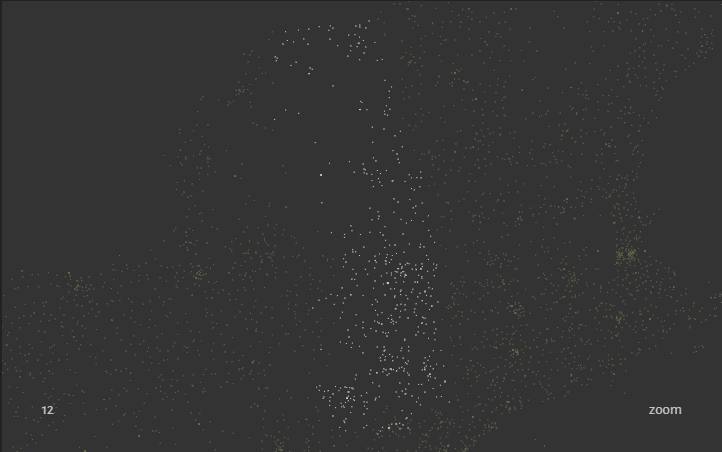
\includegraphics[scale=0.75]{chapter7/fry_zipcode3}
\caption{Zoomed In View of Fry's \cite{fry} Map }
\end{figure}

By zooming in further on the data and typing in the zipcodes gives a much more precise view of the data shown on the map as shown in Figure 7.18. It was these techniques that inspired me to try out a similar concept and achieve the same output using the Royal Mail postcode data. This data set consists of much larger rows than the US data set. The data included in this PAF file includes millions of addresses and postcodes from various locations. This includes England, Scotland, Northern Ireland, Wales, Jersey, Guernsey and the Isle of Man. The license to use the data for this experiment has been acquired from the Royal Mail accredited provider, all copyright on the data is owned by the Royal Mail Group Ltd \cite{mail1997postcode}. The postcode is part of a unique coding system designed for the sorting of mail. Invented and administered by the Royal Mail in 1974, postcodes are abbreviated forms of the whole address, and this system allows the UK to be split into designated delivery points \cite{mail1997postcode}. These could also be for a variety of other purposes - some of which include the calculation of insurance premiums, the designation of destinations in route planning software and even as the lowest level of aggregation in census enumeration. All of these purposes however, can be achieved through the breakdown and analysis of the data in a particular fashion, all of which can be done through this unique visualisation techniques.

%Figure 7.19
\begin{figure}[H]
\centering
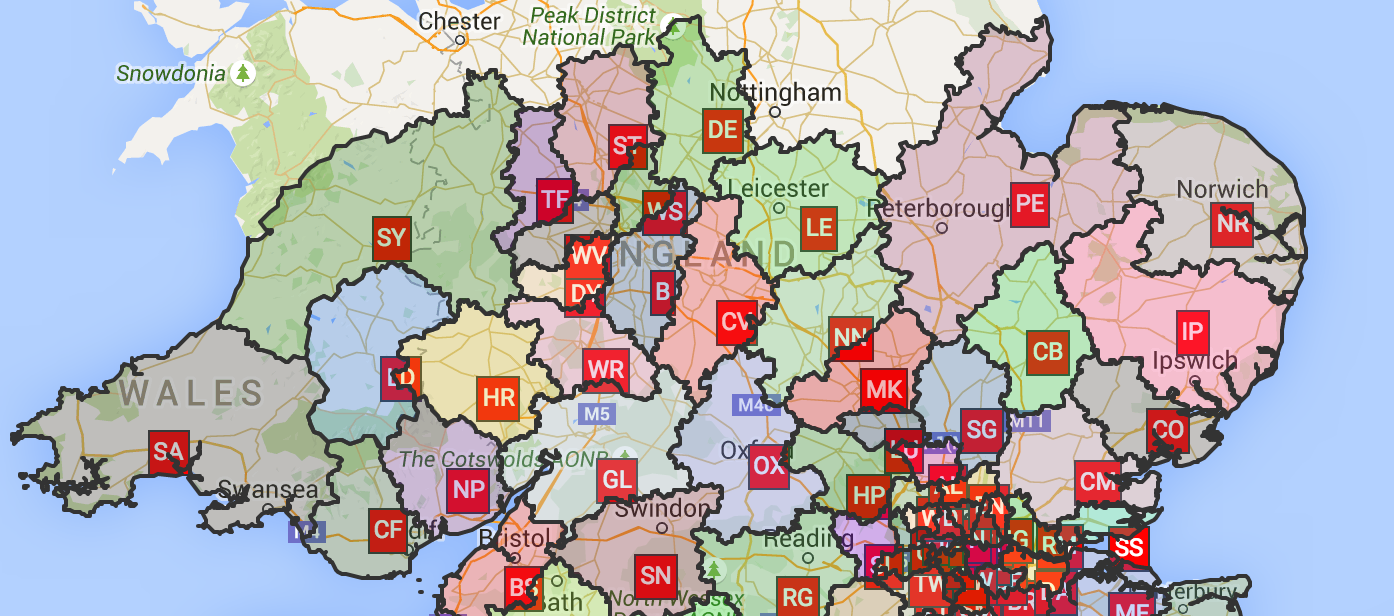
\includegraphics[scale=0.6]{chapter7/postcodenew1}
\caption{UK Postcode Visualisation Based on Postcodes}
\end{figure}

To create this graphical view a dynamic and interactive digital map for the purposes of this experiment is selected as demonstrated in Figure 7.19. The interesting thing about this type of visualisation is that the users have the ability to explore map data, finding cities and locations. This type of map also makes it much easier for standard users to understand the large Royal Mail postcode division and its related areas.

%Figure 7.20
\begin{figure}[H]
\centering
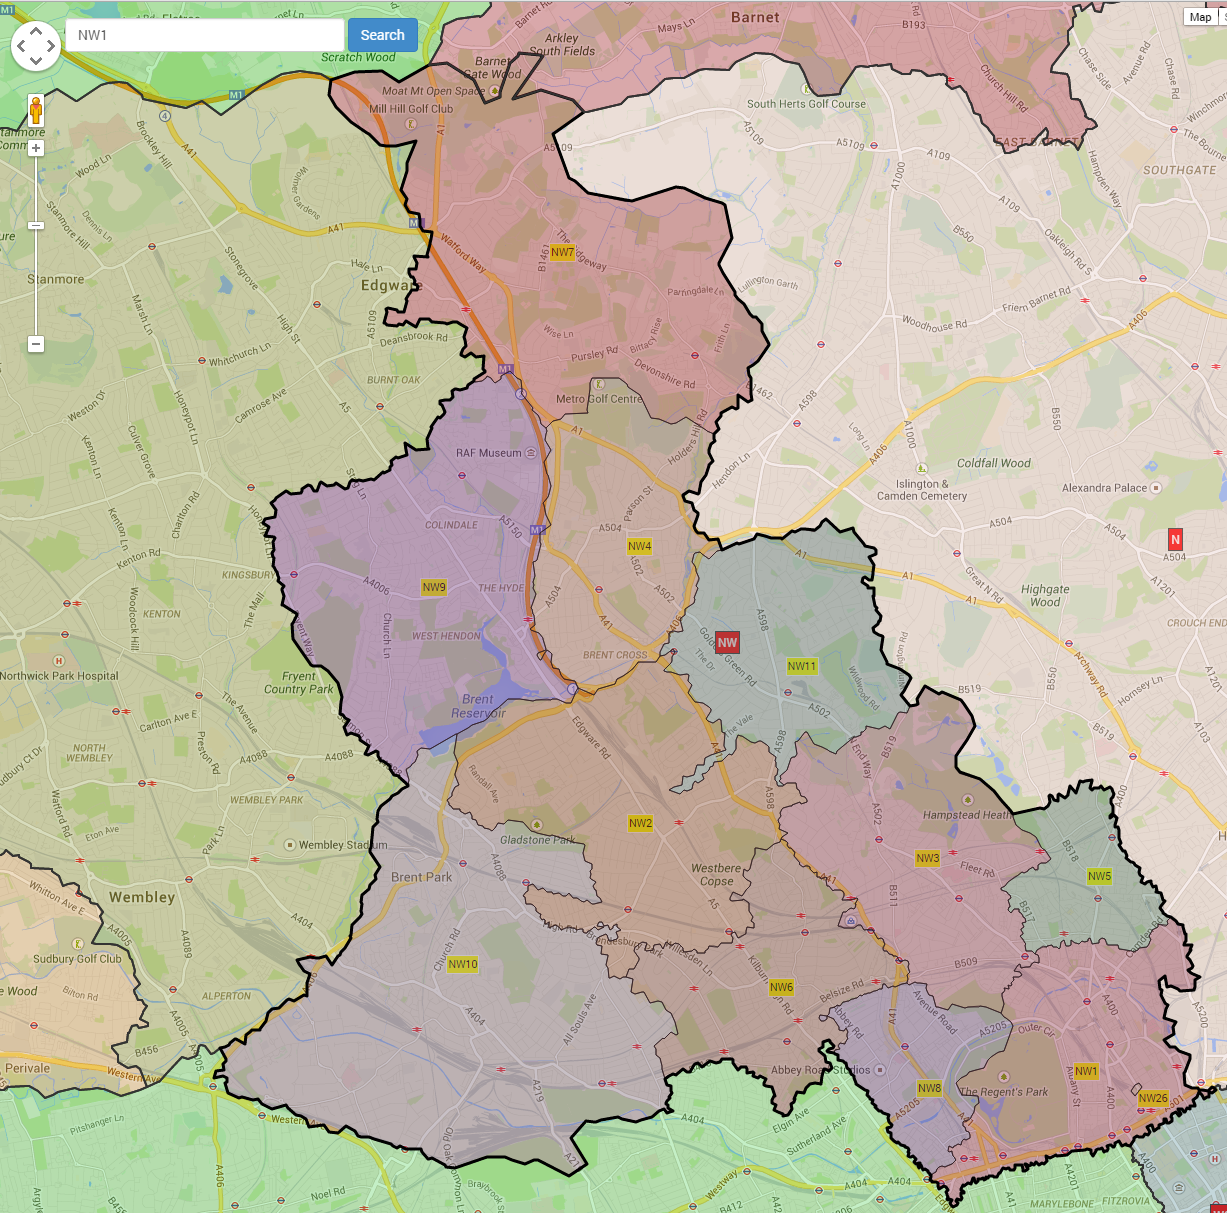
\includegraphics[scale=0.4]{chapter7/ukpostcode2}
\caption{ Zoomed In and Sub-Postcode Map}
\end{figure}

In the map demonstrated in Figure 7.20, when the postcode NW1 is entered into the search bar, the map has the ability to analyse the data and suggest a series of sub postcodes in the selected geographic area. UK postcodes are much more complex than the US zipcodes, and the number of postcodes in the UK are much higher than those in the US. But showing the sub-categorisation of the postcode data gives the user extra information, including a boundary line of areas which are simply not available in the system discussed above. These little sub categories give even more information to the user - and the system understands and compensates for that. The system used to create this interactive map is incredibly intelligent, and the new subcategories that are available are now marked with their own tags and boundaries. These are all in different colours with corresponding tags, while still remaining different from the upper levels of distinction. In this new level of interaction, a user can quickly and easily see where NW1 lies on this map. The information could be drilled down further and further, into more detail by continuing to refine the data, the searches or interacting with the system. As Figure 7.21, the further user dig, the more detailed information about the postcode can be shown on the map. It shows clearly where each postcode is located on the map, users can choose to explore interactive map further to see the street names belonging to each postcode at each address.

\begin{figure}[H]
\centering
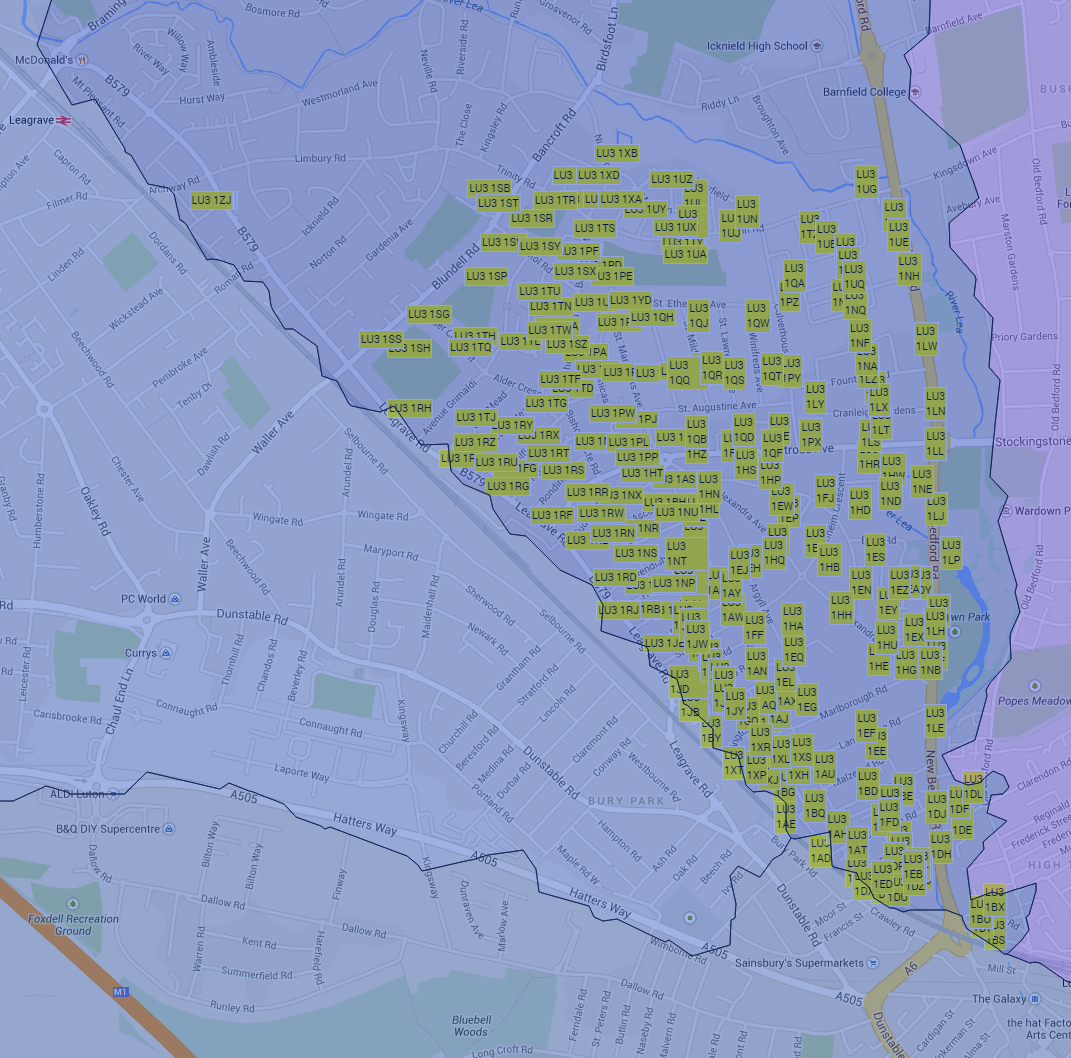
\includegraphics[scale=0.4]{chapter7/sub_postcodes2}
\caption{ Detailed / Zoomed In UK Postcode Map}
\end{figure}

The proposed system has opened up a completely new scope to complex data sets. Introducing the added features from exiting interactive maps which gives users even more intuitive information when compared to the previous approaches adopted to the same results. In Figure 7.21, a much more detailed selection of postcode data is shown - utilising the zoom function of an interactive map with up to date street information that can be made visible to customers as well as users.

\begin{figure}[H]
\centering
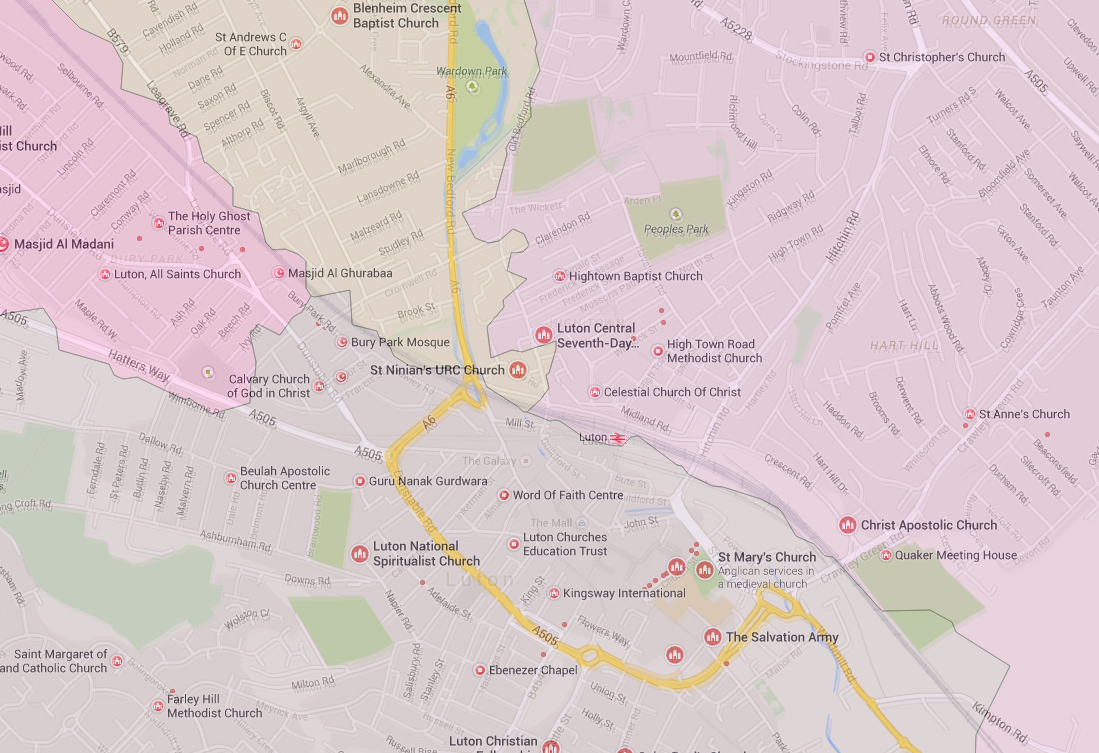
\includegraphics[scale=0.37]{chapter7/ukpostcode_church_data}
\caption{ UK Postcodes and Mosques/Churches Shown Together}
\end{figure}

These additional data sets (such as places of worship, schools or hospitals) shown in Figure 7.22, has also been merged with the postcode data from the Royal Mail data set, and these have been presented in a visualised form. This addition of data gives end users a new portal to search for places on interest in a more interactive and intuitive way.

\begin{figure}[H]
\centering
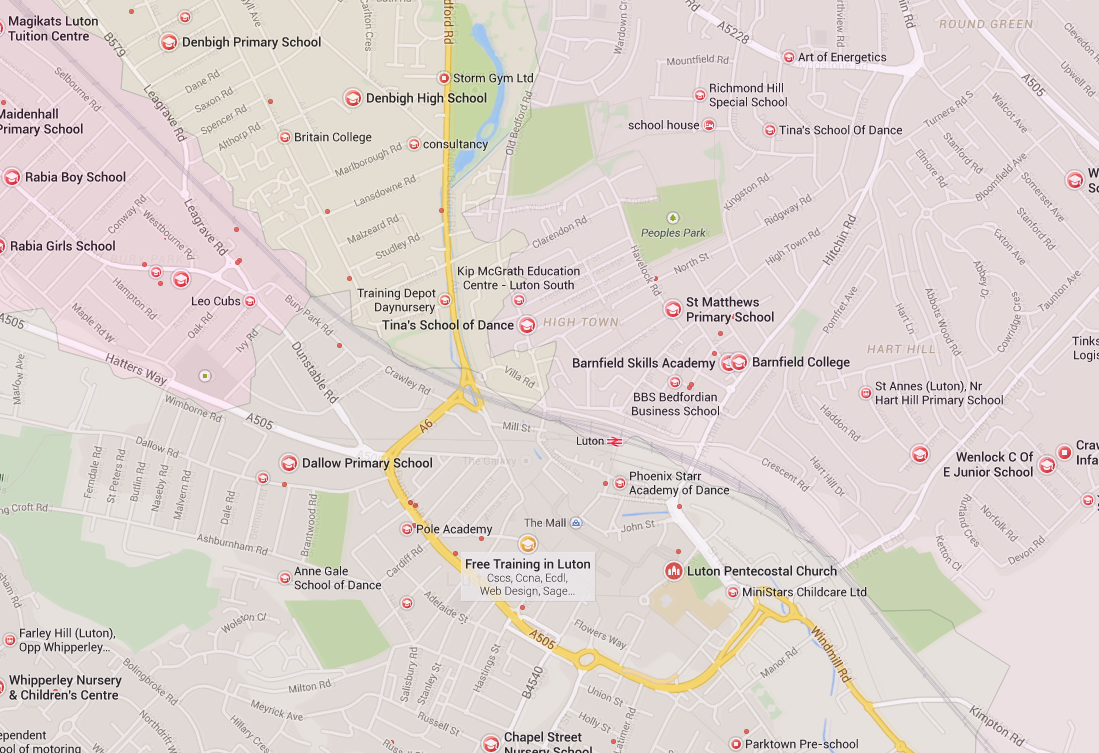
\includegraphics[scale=0.37]{chapter7/uk_postcode_schools}
\caption{ UK Postcodes and Schools/Colleges Shown Together}
\end{figure}

Educational institutes are also shown within this map illustrated in Figure 7.23, and this gives the users the unique ability to see where schools, nurseries and colleges are located on the map and in what postcode area can be found. This interactive map element processes several data sets at the same time, allowing multiple views on the data to form educated views

%Figure 7.24
\begin{figure}
\centering
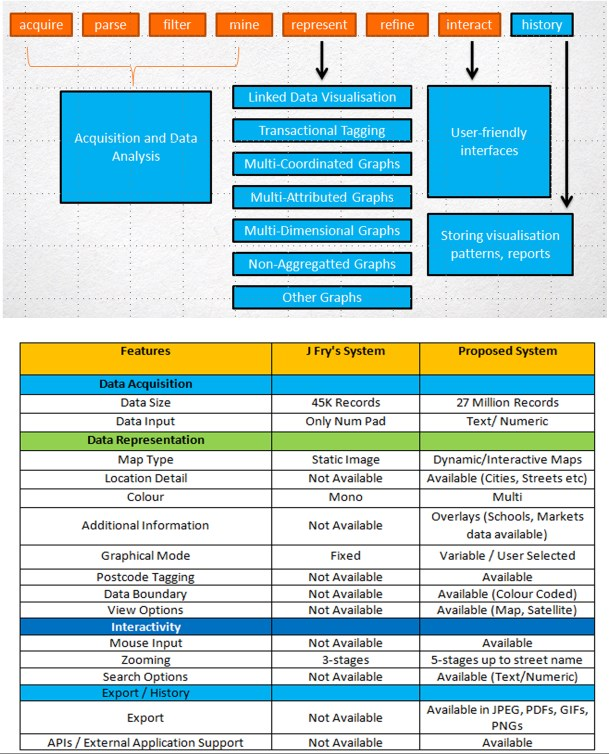
\includegraphics[scale=0.82]{chapter7/result/fry_comp}
\caption{System Comparison Table with Fry's Model}
\end{figure}

Figure 7.24 shows comparison overview of the proposed system with Fry's visualisation model \cite{fry}. The first four layers are incorporated into one layer in the proposed model called acquisition and data analysis layer. The represent++ layer is further enhanced with introduction of linked data and transactional data visualisation. Interact++ layer is equipped with new interactive mediums and visualisation approaches facilitating ease of use and friendliness of the system. Export features are incorporated at the history layer of the visualisation model. \\

The comparison is based on proposed research objectives such as acquisition and data analysis, data representation, interactivity of the system and exporting visualised content. In the geographical data set comparative analysis, zipcode data set consists of only 45K records while Royal Mail PAF (Postcode Address File) file contains millions of records. The size of PAF file was enormous. The visualised map in Fry's system is static while on the other hand, interactive map was utilised in the proposed system. Location detail such as street name, street view, town and city information was is only available in the proposed system. Additional data sets are applied in the proposed system while the other system, only analyses zipcode data set. Graphical mode is dynamic in the proposed system as user can select locations as needed. Data boundaries and postcode tags are introduced in the proposed system while these features are absent in the other system. Exporting visualised content in various formats provided in the proposed system application. The Fry visualisation system allows users to produce static visualisations of data while still being able to interact with the data. This new approach has presented data analysis techniques with a more dynamic data set and a range of interactive maps that are presenting information in a new and unique way. More than one data set can be processed at the same time allowing for a much more dynamic outcome. Visualisd content could be exported for comparison and external usage purposes. 

\subsection{System Comparison with Additional Tools}

In order to achieve data visualisation there are selection of system tools required. These tools allow users to explore the data, mine it fully and visualise it in a succinct and effective way. 

\subsubsection{Excel Charts}

Graphs, also known as charts, are incredibly useful tools for data visualisation using Microsoft Excel, users can make it quick and easy to add spreadsheets and allow the story to flow in visual form or give a presentation in a dynamic style. Studies show people are 80\% more likely to remember information that is presented in a visual format than information given aurally \cite{avons1980visualization}. Graphs might seem intimidating from first glance, are actually an incredibly simple and easy thing to do - and it can be done through a simple excel spreadsheet. In excel, users can select from many basic types of graph, plus many more advanced options, to visualise the data. Excel has an overabundance of choices when it comes to the charts and graphs - so no matter what users preference or requirement, users will find something that works. 

%Figure 7.25
\begin{figure}[H]
\centering
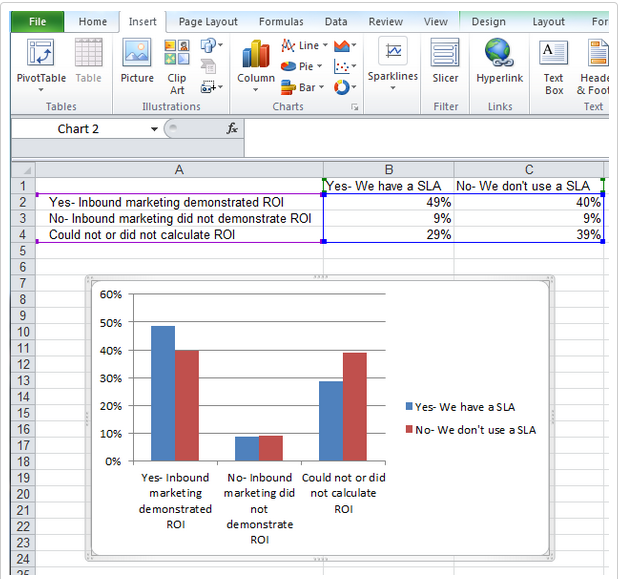
\includegraphics[scale=0.8]{chapter7/excel_charts1}
\caption{Excel Visualisation}
\end{figure}

Excel is a good tool that is used by many different small businesses and even individuals to visualise their data in easy to understand ways a simple bar chart visualisation is depicted in Figure 7.25. However, in order to visualise data using excel there is a lot of manual work required. The relevant data from the set needs to be selected manually and analysed on its own. This is where the proposed information visualisation system can make visualisation much easier - it has been intelligently designed over to make automated intelligent decisions about the data type and it's representation. On top of that, working with such large transaction data is extremely hard to do, and it makes manual selection a very tedious process, and once that is done then moving onto visualising the data, which can take even longer. All of this adds up and this can make it a daunting and undesirable task for anyone. Not only that, but excel also has a major limitation in the number of rows it can process, making it difficult to manage large data sets. On the other hand, this unique and robust system has been specifically designed to handle such high demand data easily, and this means it can manage large data sets, allowing it to be analysed by the system quickly and effectively while allowing access to the data in real time, freeing it for analysis.  

%Figure 7.26
\begin{figure}
\centering
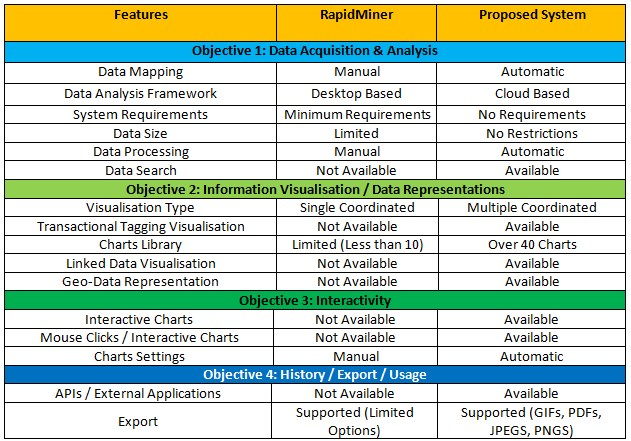
\includegraphics[scale=0.7]{chapter7/result/excel_comp}
\caption{System Comparison Table with Microsoft Excel Visualisation}
\end{figure}

Figure 7.26 illustrates comparison between Microsoft Excel and the proposed system. The comparison of these two systems is only based on data analysis and visualisation aspects. The comparison of the two systems is focused on the four key objectives of the proposed research. These objectives are highlighted as: (i) data acquisition, (ii) data representation, (iii) interactivity and (iv) history. \\

The data acquisition feature is extensively analysed in both systems. The mapping of imported data is manual in Microsoft Excel while the proposed system has algorithms for data analysis for the imported data. Data is automatically processed and mapped in the proposed system. Microsoft Excel is a desktop based application while the proposed system is a cloud based application accessed through internet browser. There are limitations on file sizes imported into Microsoft Excel while the proposed system can handle large data sets. Data search through web intelligent agents is another good feature in the proposed system while Microsoft Excel provides manual data search. The information visualisation is single coordinate while the proposed system provides multi-coordinate and multi-attribute data visualisation. Linked Data and transactional tagging techniques are not available in Microsoft Excel while the proposed system has these novel techniques which further enhances data analysis process. Geo-data representation features are not available in Microsoft Excel while the proposed system has extensive library of geo-data visualisation techniques. Graphs are not interactive in Microsoft Excel. The visualised content export features such export graph data in XML are not available in Microsoft Excel while the proposed system provides extensive solutions on data export for comparison and external usage of the visualised content.



\subsubsection{RapidMiner}

Data mining involves the exploration of data in the hope of finding the diamond of essential information for operational output. Data mining is used to analyse data, finding and dissecting the elements within the data that are useful before discarding the rest. This is done using data mining tools, which have helped to discover new knowledge, explore data from alternative perspectives, define aspects for categorisation and even summarise the complex relationships within the data sets. Data mining is often combined with statistical analysis to help understand the relationship between information within the data sets, and due to the vast amount of research done in this area there are many solutions out there to help us make sense of this complex data.

Rapid Miner is a unique software platform that has been developed by the company RapidMiner. This platform provides an integrated environment for machine learning, data mining, text mining, predictive analytics and business analytics in an efficient way. It's most commonly used for business and industrial applications, as well as for research purposes, extending educational uses, training, rapid prototyping and even application development. The RapidMiner application is desktop based with extensive data mining techniques and give users the option to visualise mined data. There are some limitation, the graphs and charts are not interactive. The process is time consuming and the business managers or users will need to learn the application before digging into data visualisation process. There are some limitation in data import as the application can't import data without binominal data. However, the Visualixer and the mashup tools utilised in this research has extensive library of interactive graphs and charts. The whole process of data import is much simpler with cloud based application. There is no binominal limitation on data import in the Visualixer. The proposed model and Visualixer mashup tool as have API access to external application fo the ease of integration. However, the whole process is extremely easy and fast while such elements are lacking in RapidMiner. 

%Figure 7.27
\begin{figure}[H]
\centering
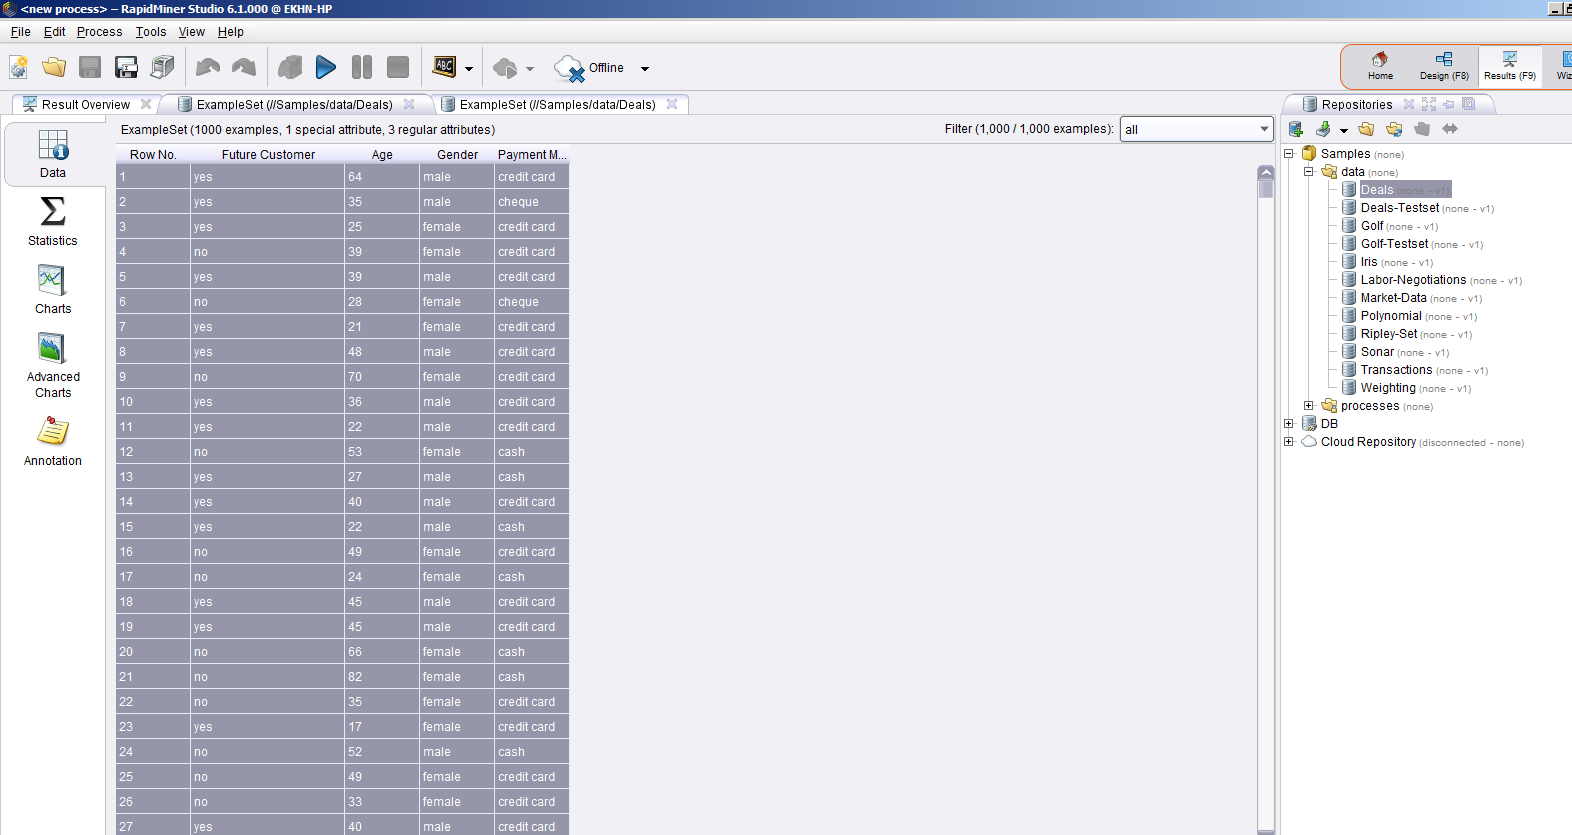
\includegraphics[scale=0.3]{chapter7/rapidminor/data_screen}
\caption{Data Overview in RapidMiner}
\end{figure}

\begin{figure}[H]
\centering
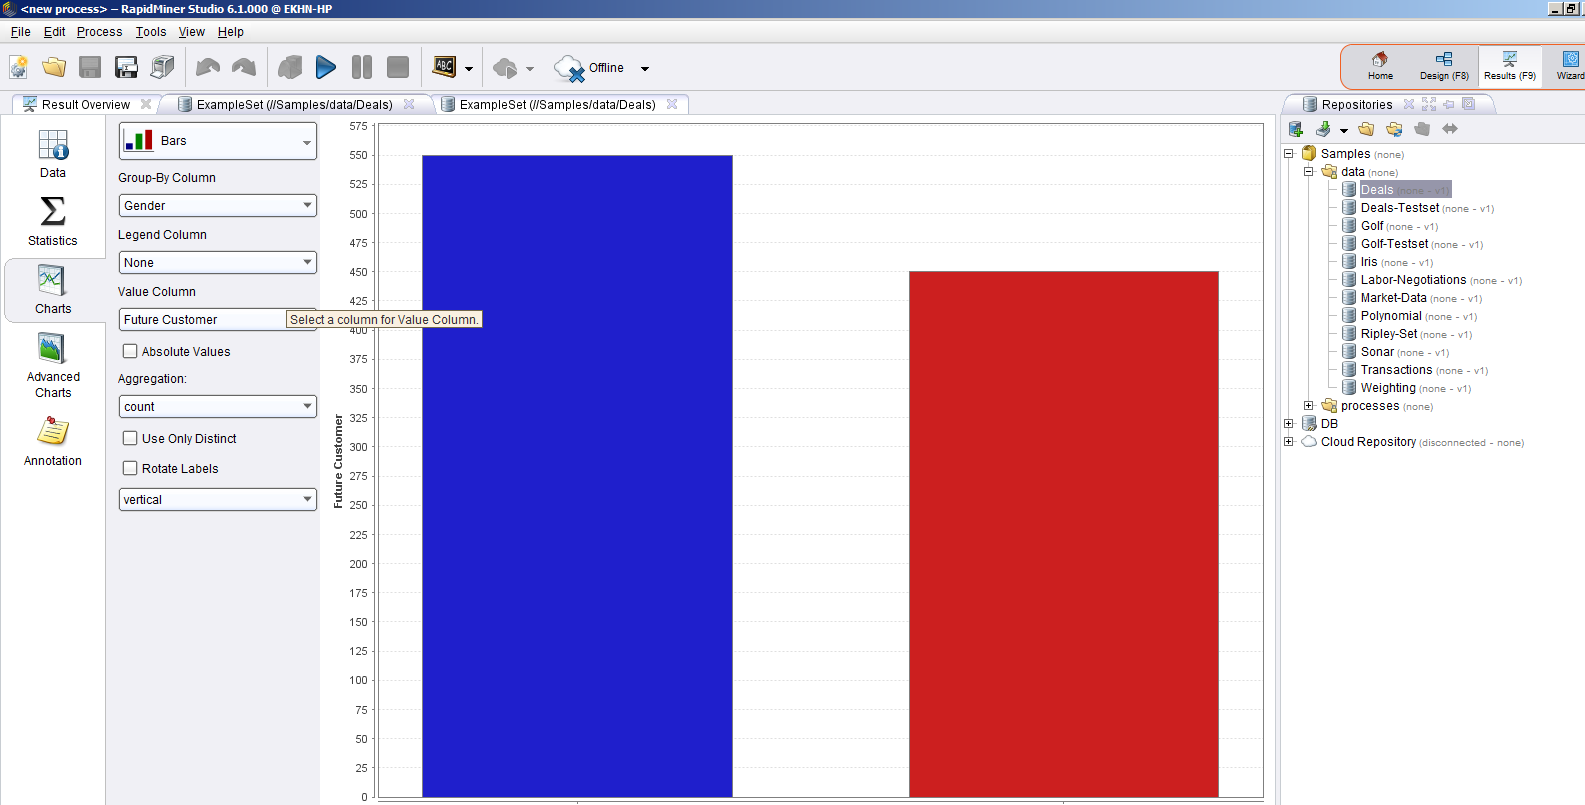
\includegraphics[scale=0.3]{chapter7/rapidminor/visualisation}
\caption{Data Visualised in RapidMiner}
\end{figure}

%Figure 7.29
\begin{figure}[H]
\centering
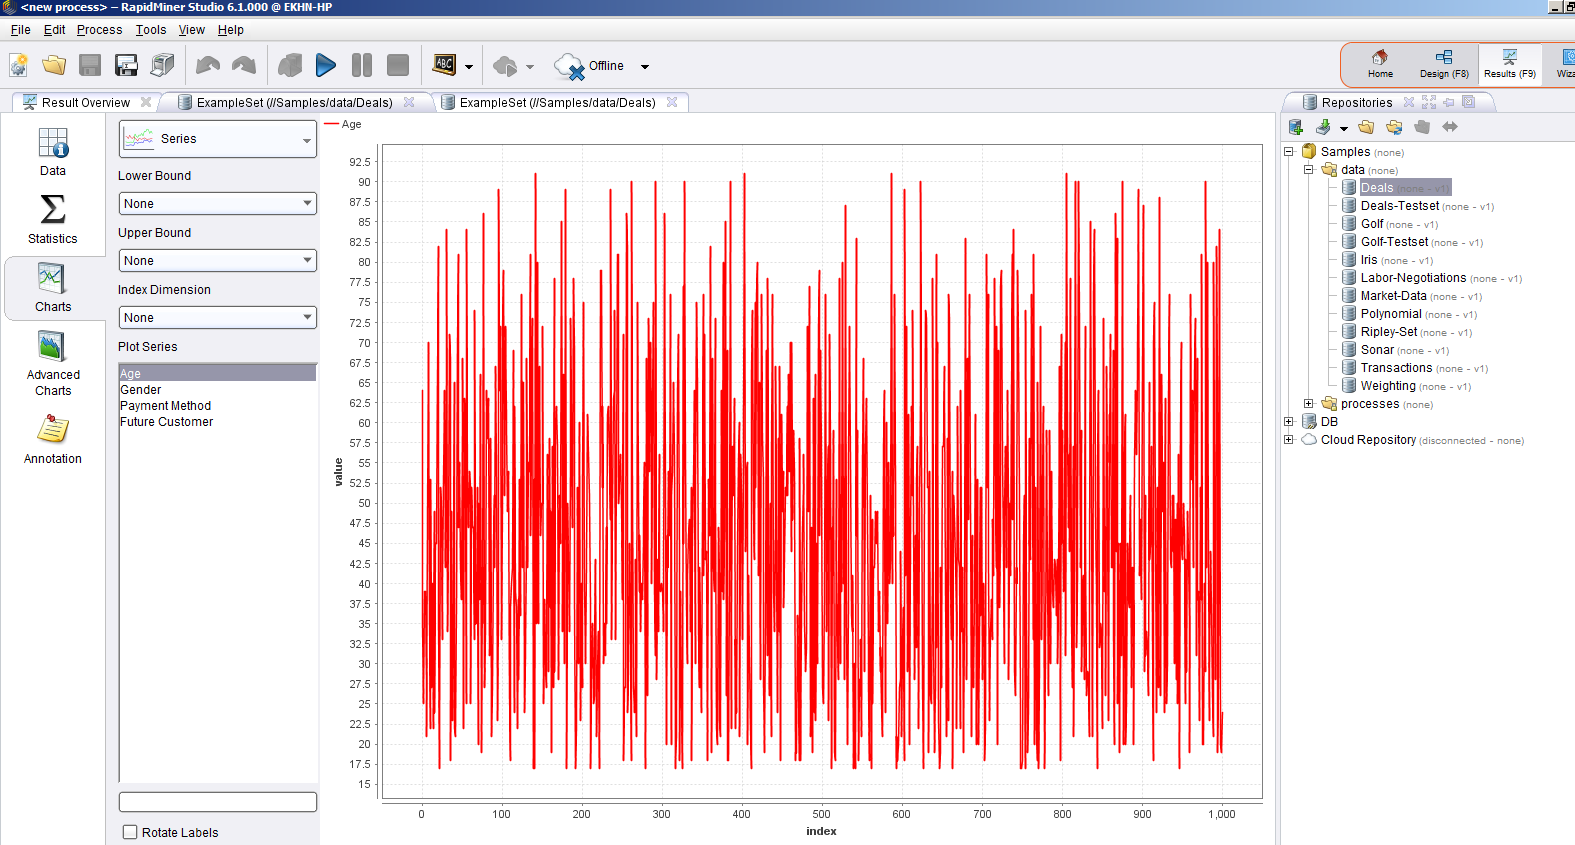
\includegraphics[scale=0.3]{chapter7/rapidminor/visualistaion2}
\caption{Different Style - Same Data Visualisation}
\end{figure}

Figure 7.27 shows the data import process in RapidMiner application. The data import feature in RapidMiner is quite compressive. RapidMiner gives various import options to users such as CSVs and XML. The system facilitate users to design and review imported data. The data import process takes a couple design steps (selection options) before it could be visualised. Figure 7.28 depicts a simple bar chart visualisation in the RapidMiner application. The left hand side menu bar shown in Figure 7.29, gives more options to users, where different styles of visualisation could be selected such as pie charts, scatter charts and area charts. The left-side menu bar also gives grouping and vertical or horizontal visualisation options. The data series graph shown in Figure 7.29 is another type of visualisation for the same data. The data series is created based on line graphs. RapidMiner is a desktop application and require good resources and intermediate skills to operate. The charts visualised are not interactive, while the output is only in static images. The same process is done through Visualixer, which is a cloud based visualisation tool developed for the proposed research. Visualixer has an easy interface in importing data and the raw data is visualised in two simple steps, with further refinement and graphs selection given at the interact++ layer. \\

%Figure 7.30
\begin{figure}
\centering
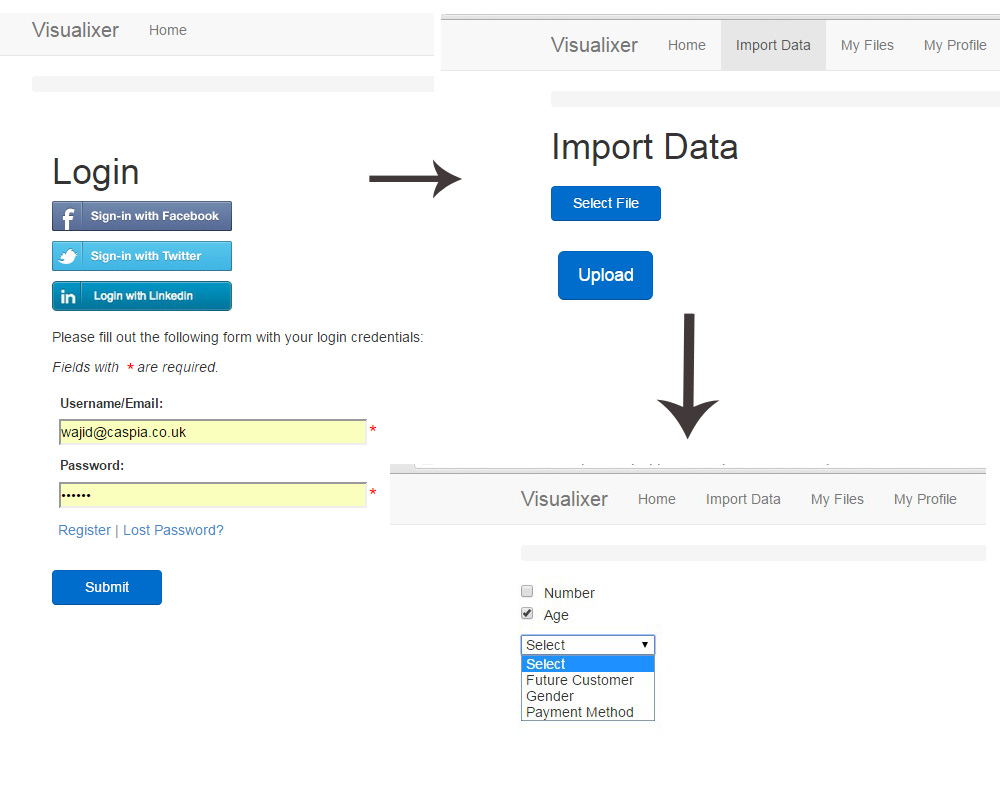
\includegraphics[scale=0.3]{chapter7/rapidminor/3steps_vis}
\caption{Sign Up, Data Import, Data Selection Steps in Visualixer}
\end{figure}

The sign up, data import and data selection process is illustrated in Figure 7.30. The users are given options to sign up with social media accounts such as Facebook, Twitter and Linkedin or with an email address. After the sign up process, users are given options to upload data set. The upload option is quite simple as shown in Figure 7.30. The browse file option is given while uploading data set files into the Visualixer data analysis tool.\\

%Figure 7.31
\begin{figure}
\centering
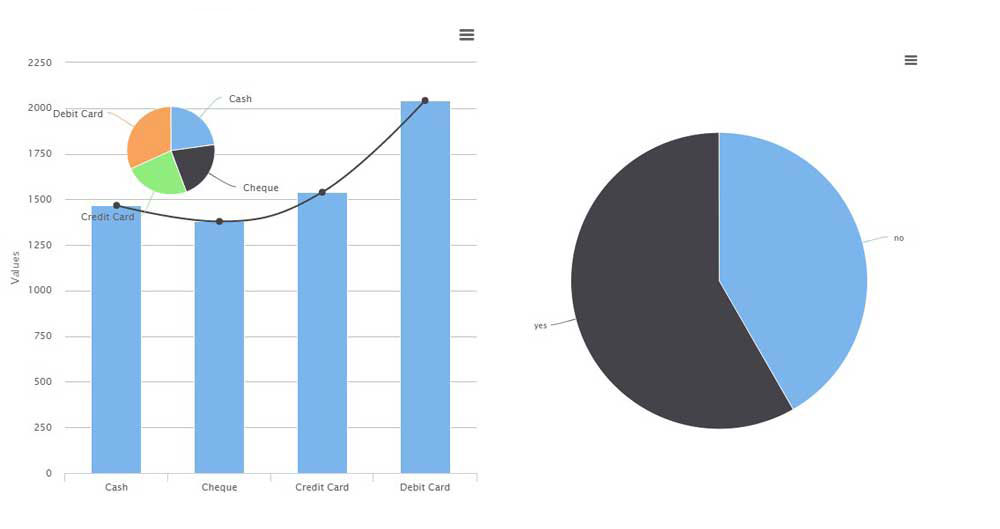
\includegraphics[scale=0.4]{chapter7/rapidminor/multi_vis}
\caption{Multi-attribute Data Visualisation in Visualixer}
\end{figure}

Figure 7.31 shows multi-attribute data visualisation, a feature which is missing in Rapid Miner, also all the charts are interactive, giving additional information on hover. These features gives a new dimension to information visualisation. Figure 7.32 shows multi-coordinate visualisation, where same data is visualised in two different styles which helps users with indepth data analysis. Visualixer enable users with a rapid registration and sign up process. The data acquisition and analysis process is fast and robust. The system is able to analyse complex data elements on the go and provide options to users to select data attributes which needs to be visualised. Visualixer helps users to analyse data in a multi-coordinate visualisation along with multi-attribute visualisation. Exporting results give an extra edge to the tool. As visualised data could be exported in various formats for comparison and external usages.\\

%Figure 7.32
\begin{figure}
\centering
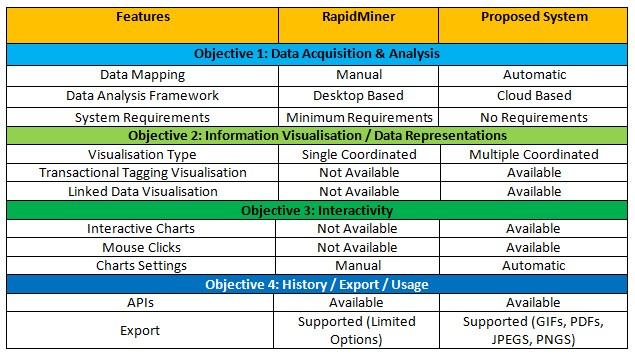
\includegraphics[scale=0.8]{chapter7/result/rapidminer_comp}
\caption{System Comparison Table with RapidMiner Visualisation}
\end{figure}

Figure 7.32 shows comparison between RapidMiner and the proposed system. Comparison is based on the four important objectives of the proposed research. The selected objectives are (i) data acquisition, (ii) data representation, (iii) interactivity and (iv) history. The first objective of the research looks into data import procedures. The data mapping in RapidMiner is manual while it is automatically processed by the proposed research system. RapidMiner is a desktop based data mining tool while proposed system is a cloud based system accessible from anywhere in the world through internet and a browser. There are minimum requirements for RapidMiner installation while no installation required for the proposed visualisation system. RapidMiner provides various visualisation styles but linked data visualisation and transactional tagging visualisation approaches are supported by RapidMiner. Graphs are interactive in the proposed system along with mouse clicks while these features are not extensive developed in RapidMiner. The proposed system provides visualised content export features in various formats such as PDfs, JPEG, GIF, XML etc. The export features in RapidMiner are limited.

\section{System Evaluation Through Survey}

The proposed system was validated through various extensive experiments explained in chapter 5, 6 and 7. However, further evaluation was undertaken through user acceptance tests. Various methods methods were explored in evaluating system usability and friendlies. These methods are briefly highlighted below.

Hallway testing is a usability test set-up in a high foot traffic area, utilising bystanders to test your product. Your participants will be people who happen to be walking down the hall and are able to afford 5-10 minutes of their day \cite{hallway}. User friendliness and usability of any system is an important process. The focus in such practices is on how easy user interfaces are to use. The term usability refers to ease of use approaches which are utilised during design process of any application. Usability is defined by 5 quality components \cite{nielsen1994usability}. These components are divided into 5 areas, which are explained below.

\begin{itemize}
\item 
Learnability: How easy is it for the user to accomplish basic tasks while using the system for the first time? 
\item	Efficiency: Once users understand system function, how easy is it for them to perform various tasks.
\item Memorability: If the users have not used the system for a while, how easily can they re-establish proficiency?
\itme Errors: How many errors do users make, how severe are these errors, and how easily can they recover from the errors?
\item Satisfaction: How pleasant is it to use the design?

\end{itemize}

Usability and user satisfaction are incorporated into the user requirements and into research objectives. The system allows  users the choice of different visualisation styles as it is not static or fixed. The system has a library of many different visualisation styles; the user is given the option to select what is more meaningful or understandable to them. There are single coordinated visualisations for staff users and more graphical data representations for managers and administration. The different levels of user requirements were incorporated while designing the visualisation model. The usability and user interaction aspects are tackled at the interact++ layer. The following user requirements are considered:
\begin{itemize}

\item 	Visualisations must represent all the most common types of information: one-, two and three-dimensional; multi-dimension data;
\item 	Users must be able to control which visualisation styles are used during a data exploration session;
\item 	Users should be able to use a range of different visualisation styles in a single visualisation package rather than be forced to use several packages;
\item 	The visualisation system must provide a generic set of tools that can be applied to a wide variety of visualisations, such as: requesting an overview, filtering out uninteresting items, zooming in to items of interest and requesting more detailed information;
\item 	Users must be able to select data from one visualisation style and generate a new visualisation of the selected data in the same style or a different style.
\end{itemize}

All the above key aspects are considered while developing the proposed information visualisation system. The evaluation is further extended through a comprehensive survey explained in the next section.

\subsection{User Acceptance Test}

What causes people to accept or reject information technology? Among the many variables that may influence system use, previous research suggests four determinants which are especially important. The usability and friendliness survey design is based on Lund's measuring usability technique \cite{lund2001measuring}. This technique is quite comprehensive in measuring application's user friendliness and ease of use attributes.

\textbf{Usefulness}

Firstly, people tend to use or not use an application to the extent they believe it will help them perform their job more efficiently. Table 7.1 highlights questions which will be asked from various users regarding the proposed application.


\begin{table}
\begin{center}
\begin{tabular}{ |l| } 
 \hline
1.	It helps me to be more effective. \\ 
2.	It helps me to be more productive. \\
3.	It is useful.  \\
4.	It gives me more control over the activities in my life.  \\
5.	It makes the things I want to accomplish easier to achieve. \\
6.	It saves me time when I use it.\\
7.	It meets my needs. \\
8.	It does everything I would expect it to do. \\  

 \hline
 \end{tabular}
 \caption{Usefulness Questionnaire}
\label{table:1}
\end{center}
\end{table}

\textbf{Ease of Use}

Secondly, even if potential users believe that a given application is useful, they may at the same time believe that the system is too hard to use and that the performance benefits of usage are outweighed by the effort of using the application. That is, in addition to usefulness, usage is theorised to be influenced by ease of use. The system ease of use attribute is further analysed and evaluated through questionnaire in Table 7.2.

\begin{table}
\begin{center}
\begin{tabular}{ |l| } 
 \hline
9.	It is easy to use. \\
10.	 It is simple to use. \\
11.	 It is user friendly. \\
12.	 It requires the fewest steps possible to accomplish what I want to do with it.\\
13.	It is flexible. \\
14.	 Using it is effortless. \\
15.	 I can use it without written instructions. \\
16.	I do not notice any inconsistencies as I use it.\\
17.	 Both occasional and regular users would like it.\\
18.	I can recover from mistakes quickly and easily.\\
19.	 I can use it successfully every time.\\
 \hline
 \end{tabular}
 \caption{Ease of Use Questionnaire}
\label{table:2}
\end{center}
\end{table}

\textbf{Ease of Learning}

Thirdly, how easy is the system to use -  how quickly did users learn to operate the system -  is it memorable or difficult to operate? Such attributes and features will be analysed through questions in Table 7.3.

\begin{table}
\begin{center}
\begin{tabular}{ |l| } 
 \hline
20.	I learned how to use it quickly.\\
21.	I can easily remember how to use it.\\
22.	It is easy to learn.\\
23.	I can quickly become skilful with it.\\
 \hline
 \end{tabular}
 \caption{Ease of Learning Questionnaire}
\label{table:3}
\end{center}
\end{table}


\textbf{Satisfaction}

Whether users are satisfied with the application or not, will they recommend it to other businesses or friends;  is it fun to use, and is it an overall pleasant experience or not? Table 7.4 will measure user's satisfaction aspects.

\begin{table}
\begin{center}
\begin{tabular}{ |l| } 
 \hline
24.	I am satisfied with it.\\
25.	I would recommend it to a friend.\\
26.	It is fun to use.\\
27.	It works the way I want it to work.\\
28.	It is wonderful.\\
29.	I feel I need to have it.\\
30.	It is pleasant to use.\\
 \hline
 \end{tabular}
 \caption{Satisfaction Questionnaire}
\label{table:4}
\end{center}
\end{table}

\subsection {Survey Results}

This survey was useful and gave an indication of the system’s usefulness and the ease of use. The survey also provided a comprehensive list of pros and cons of the application in tackling the data problem. The survey was conducted in 9 different companies and 135 staff members participated. All of the users who participated in this survey utilised the application developed through the proposed research model. The survey results are classified as below.

\textbf{Usefulness}

Table 7.5 shows survey results based on the usefulness of the application. The questionnaire was based on 5 radio buttons, where 1 shows disagreement while 5 shows strong agreement. The survey results based on the usefulness of the application.\\

%Figure 7.33
\begin{figure}
\centering
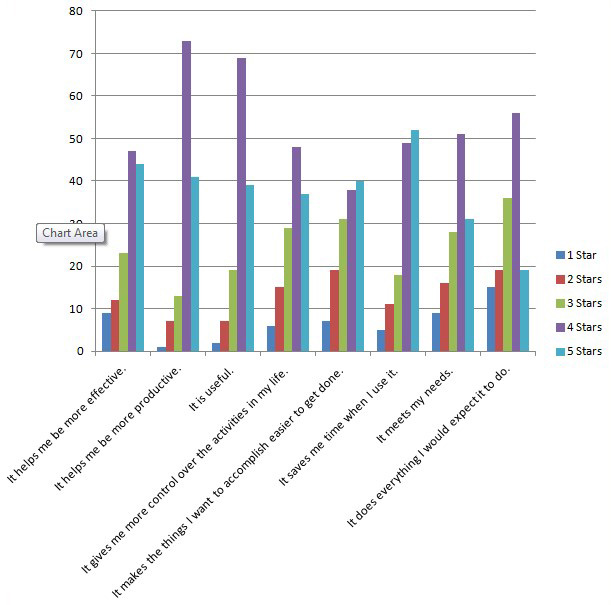
\includegraphics[scale=0.68]{chapter7/result/usefulness_chart}
\caption{System Usefulness Survey Result Graph}
\end{figure}

There were only 54 1-star ratings for the 8 questions in the usefulness questionnaire. That is only 4\% of the users showing less confidence in the usefulness of the application. There were only 106 2-star responses from the 8 usefulness questions. That is only a 9\% rating at 2-star. There were 197 3-star responses to the 8 questions. That makes around 18\% at the 3-star response, which is just average. There were 431 4-star responses to the 8 questions, which makes 39\% ratings at 4-star, which is well above average. There were 303 responses at the 5-star rating, showing that 28\% of the users consider the application to be extremely useful for the activities and tasks. To summarise, 28\% and 39\% (4 and 5 – star ratings) of the users consider the application to be very useful as shown in Table 7.5. 

\begin{figure}
\centering
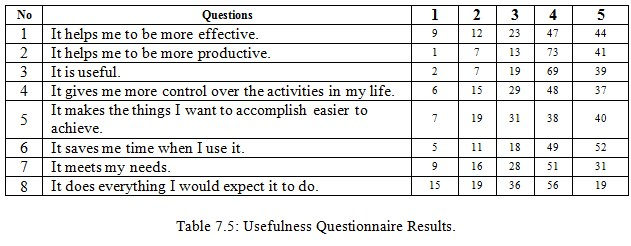
\includegraphics[scale=0.8]{chapter7/result/result1}
\end{figure}

The chart in Figure 7.33  demonstrates the survey results. The legend 1 star shows strong disagreement while 5 stars show strong agreement. \\

\textbf{Ease of Use}

In this section, application usage in terms of user knowledge and understanding is measured. There were 11 questions asked in this block; all of these questions are related to the system usage and ease of use. The results are further visualised in Figure 7.34.\\

%Figure 7.34
\begin{figure}
\centering
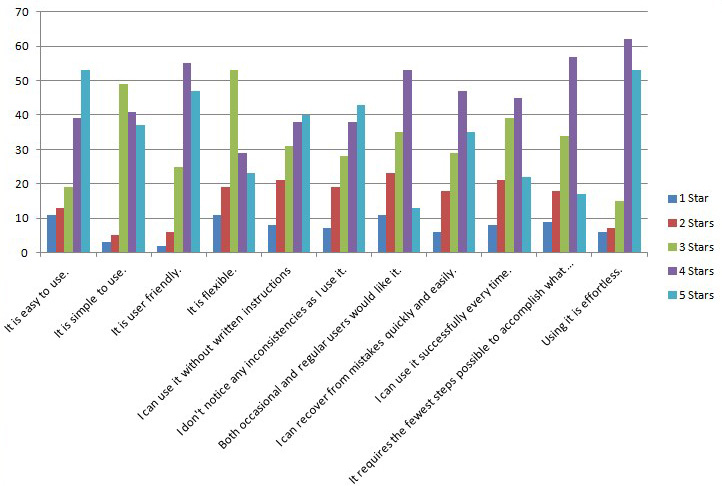
\includegraphics[scale=0.58]{chapter7/result/ease_of_use}
\caption{System Ease of Use Survey Results}
\end{figure}

\begin{figure}
\centering
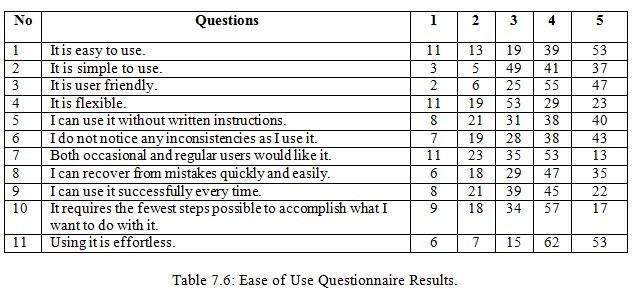
\includegraphics[scale=0.8]{chapter7/result/result2}
\end{figure}

There were 82 responses to all the questions in the 1-star column, which shows that only 6\% of the users who used the system consider the system to be very complicated. There were 170 responses to the 11 questions at the 2-star rating, which suggests that 11\% of the users believe the application is complicated and not easy to use. There were 342 responses in the 3-star column,  suggesting that 23\% of the users believe the system is easy to use. There were 504 submissions on the 4-star column to all the questions in the easy to use block, suggesting that 34\% of the users have found the system very easy to use. There were 383 responses to the 5-star category, which highlights that 26\% of the users found the system extremely easy to use. The responses in the 4-star and the 5-star columns (34\% and 26\%) suggest that the system is very easy to use as shown in Table 7.6 .\\

\textbf{Ease of Learning}

The third part of this survey has four questions; this block of questions is more focused on aspects such as how easy the system is to learn and utilise without referring to the operating manual. The table below, along with the chart in Figure 7.35, highlights the survey results based on ease of learning. \\

%Figure 7.35
\begin{figure}
\centering
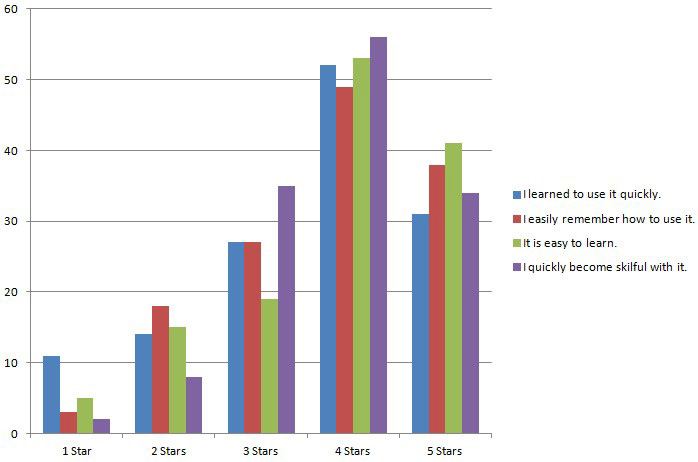
\includegraphics[scale=0.56]{chapter7/result/Ease_of_learning}
\caption{System Ease of Learning Survey Results}
\end{figure}

\begin{figure}
\centering
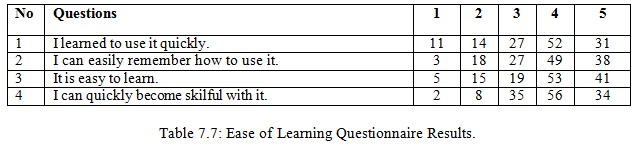
\includegraphics[scale=0.8]{chapter7/result/result3}
\end{figure}

There were 21 responses to the four questions in the ease of learning block as shown in Table 7.7. The responses suggest that 4\% of the users did not find the application easy to learn. There were 55 responses in the 2-star category, i.e. around 10\% of the users ranked the application reasonable. 108 responses in the 3-star category shows that 20\% of the users were satisfied with ease of learning. 210 and 144 in the 4-star and 5-star categories suggests that 39\% and 26\% of the users who participated in the survey were extremely happy with ease of learning while utilising different features of the system.\\

\textbf{Satisfaction}

Finally, to show how satisfied users were with the application. There were 29 responses to all the questions in the ratification questionnaire block in the 1-star category as shown in Table 7.8; this shows that only 3.5\% of the users were not satisfied with the application at all. There were 77 responses in the 2-star category, so around 10\% of users showed signs of satisfaction but were not really impressed with the applications and the proposed system approach. There were 174 responses in the 3-star question block so around 21\% of the users were reasonably satisfied with the system. 310 voted in the 4-star category, which shows that 38\% were satisfied with the system features and outputs. 218 responses were recorded in the 5-star category, which shows that 27\% of the users were extremely satisfied with the application's efficiency and output. 

%Figure 7.36
\begin{figure}
\centering
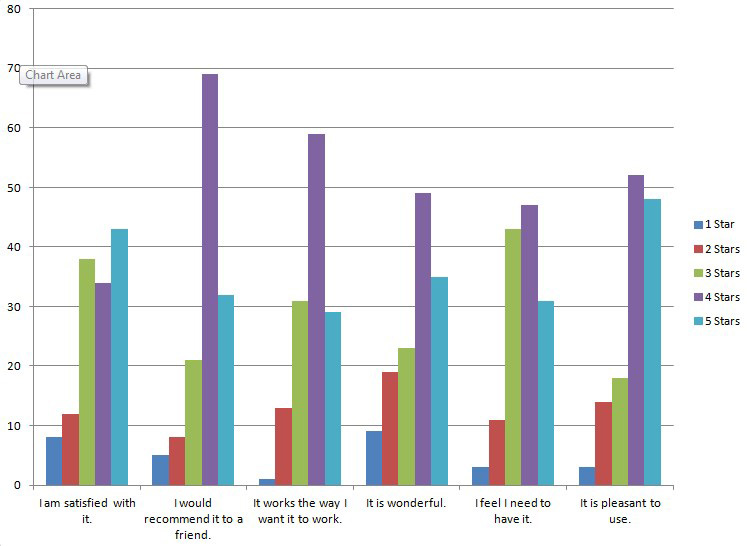
\includegraphics[scale=0.55]{chapter7/result/satisfaction}
\caption{System Satisfaction Survey Results}
\end{figure}

\begin{figure}
\centering
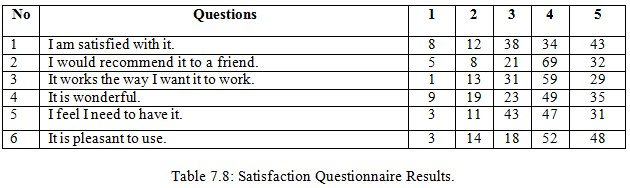
\includegraphics[scale=0.82]{chapter7/result/result4}
\end{figure}

\textbf{Conclusion}

Table 7.9 captures the users’ acceptance in various blocks. The survey average results are displayed in three different categories from one extreme to the other (not satisfied to extremely satisfied). Table 7.9 suggests that only 7\% of the users did not show any interest in the four blocks of questionnaire; in other words they did not find the system useful, easy or memorable and that is why they were not satisfied. 21\% of the users in the above four different categories showed interest but they were not satisfied or disappointed. The response was average as shown in Table 7.10. Table 7.11 shows that 34\% of the users were extremely satisfied with the system’s usefulness, ease of use, ease of learning and were overall satisfied with the application and its output in enhancing efficiency and productivity.  


\begin{figure}
\centering
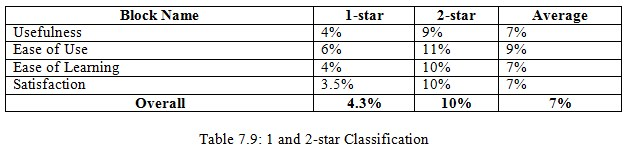
\includegraphics[scale=0.9]{chapter7/result/result5}
\end{figure}

\begin{figure}
\centering
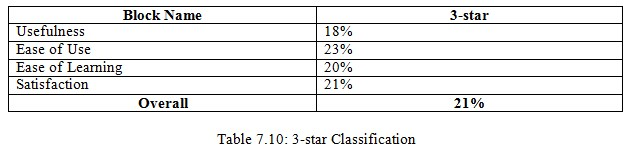
\includegraphics[scale=0.95]{chapter7/result/result6}
\end{figure}

\begin{figure}
\centering
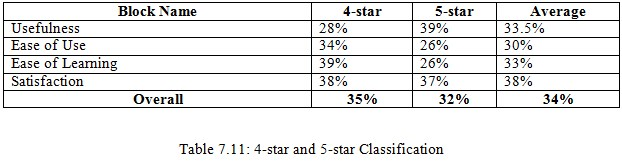
\includegraphics[scale=0.8]{chapter7/result/result7}
\end{figure}


\section{Summary}

The four layers of information visualisation model has been revisited with different perspective as multi-coordinate, multi-attribute, multiple dimension, transactional tagging and linked data visualisation explained and validated by various examples. These features are novel and solid contribution to the field of information visualisation in enterprise and Web 2.0 environment through data mashup technologies. The model and results are compared with Fry's \cite{fry} information computational model and with various other existing information visualisation tools and techniques. The research objectives are discussed and validated through different experiments. The closing remarks, research contribution, system scope and limitation are discussed in the next chapter.







